\chapter[Time evolution of CR particles]{Time evolution of cosmic ray particles from an accelerator} \label{sec:07_particle_ev}

Cosmic Rays (electrons and protons) are accelerated by sources such as PWNe and SNRs. Cosmic rays then escape the acceleration regions and subsequently propagate through the interstellar medium, losing energy through various processes such as radiative cooling, adiabatic expansion and ionisation as discussed in \autoref{sec:chapter1_non_thermal_emission}. By modelling the transport of cosmic-ray particles from an accelerator, the subsequent gamma-ray distribution can be predicted (see \autoref{sec:chapter1_non_thermal_emission}) and compared to observations.
\par~\par
This section first discusses how the energy distribution of cosmic rays evolves in time due to radiation losses and predicts the subsequent gamma-ray emission. This will then be expanded to include the escape of cosmic rays out of the region of interest due to diffusion (see \autoref{chapter_1_cr_propagation}). Finally, this section describes the numerical code developed by \cite{fabien}, which can be used for systems where the cosmic-ray energy distribution and the gamma-ray SED cannot be solved analytically.
\par~\par
This code was applied to investigate the origin of the $\GeV$ gamma-ray emission to the south of \mbox{HESS\,J1825-137}. Proposed sources included the impulsive SNR and continuous PWN associated with \mbox{HESS\,J1825-137} and the impulsive SNR and continuous compact object binary associated with \mbox{LS\,5039}. The results of this study were published in the Monthly Notices of the Royal Astronomical Society and is shown in \autoref{sec:08}.

\section{Radiation losses} \label{sec:chapter_7_cr_SED_evol} 

First consider cosmic rays being injected by a homogeneous source into a region of interest at rate $S\qty(\gamma,t)$ and escaping at rate $v_\text{esc}$. The time evolution of the cosmic-ray energy density distribution, $n\qty(\gamma,t)$, can be described by \citep{1980gbs..bookR....M}:
%The time evolution of the cosmic ray energy distribution, $n\qty(\gamma,t)$ for a homogeneous source injecting particles at rate $S\qty(\gamma,t)$ and escape rate $v_\text{esc}$ can be described by \citep{1980gbs..bookR....M}:

\begin{equation}
    \begin{aligned}
    \pdv{n\qty(\gamma,t)}{t}&=\pdv{ }{\gamma}\qty[\dot{\gamma}\qty(\gamma)n\qty(\gamma, t)] - \nu_\text{esc}\qty(\gamma)n\qty(\gamma,t) + S\qty(\gamma, t)\text{ ,}
    \end{aligned} \label{eq:chapter_7_cr_energy_distribution}
\end{equation}
\noindent where cosmic rays with Lorentz Factor $\gamma$ continuously lose energy at rate $\dv{\gamma}{t}=\dot{\gamma}$ and have probability $v_\text{esc}\dd{t}$ of escaping the system in time $\dd{t}$. Physically, $\dot{\gamma}\qty(\gamma)n\qty(\gamma,t)$ is the number of cosmic rays per unit time that cool at Lorentz factor $\gamma$ for a cosmic-ray density $n$. The following will describe the solution of \autoref{eq:chapter_7_cr_energy_distribution} using Laplace transformations.
\par~\par
Laplace transformations are used to reduce differential equations conveniently into an algebraic equation. The Laplace Transform for the function $f\qty(t)$ is given by:

\begin{equation}
    \begin{aligned}
        \bar{f}\qty(q)&=\int_0^\infty e^{-qt}f\qty(t)\dd{t}\text{ .}
    \end{aligned}
\end{equation}
\noindent Similarly, the Laplace transformation for $f'\qty(t)=\dv{f}{t}$:

\begin{equation}
	\begin{aligned}
		\bar{f}'\qty(q)&=q\bar{f}\qty(q)-f\qty(0)\text{ .}
	\end{aligned}
\end{equation}
\noindent Hence, the Laplace transformation of \autoref{eq:chapter_7_cr_energy_distribution}:

\begin{equation}
    \begin{aligned}
        q\bar{n}\qty(\gamma, q)-n\qty(\gamma,0)&=\pdv{}{\gamma}\qty[\dot{\gamma}\qty(\gamma)\bar{n}\qty(\gamma, q)] - \nu_\text{esc}\qty(\gamma)\bar{n}\qty(\gamma,q) + \bar{S}\qty(\gamma, q) \\
        -\bar{S}\qty(\gamma,q)-n\qty(\gamma,0)&=\pdv{}{\gamma}\qty[\dot{\gamma}\bar{n}\qty(\gamma,q)]-\qty[q+\nu_\text{esc}\qty(\gamma)]\bar{n}\qty(\gamma,q)\text{ .}
    \end{aligned} \label{eq:chapter_7_cr_energy_distribution_transform}
\end{equation}
\noindent The variable $Q\qty(\gamma,q)=\dot{\gamma}\bar{n}\qty(\gamma,q)$ is defined such that \autoref{eq:chapter_7_cr_energy_distribution_transform} becomes:

\begin{equation}
    \begin{aligned}
        -\bar{S}\qty(\gamma,q)-n\qty(\gamma,0)&=\pdv{}{\gamma}Q\qty(\gamma,q)-\qty[q+\nu_\text{esc}\qty(\gamma)]\frac{Q\qty(\gamma,q)}{\dot{\gamma}}\text{ ,}
    \end{aligned}  \label{eq:chapter_7_cr_energy_distribution_transform2}
\end{equation}
\noindent $Q\qty(\gamma,q)$ can be described as the number of cosmic rays per unit time that cool from Lorentz factor $\gamma$. The differential equation describing the time evolution of the cosmic-ray energy density distribution has been reduced to a first order linear differential equation of form:

\begin{equation}
	\begin{aligned}
		b\qty(x)&=\dv{y}{x}+a\qty(x)y\text{ ,}
	\end{aligned}
\end{equation}

\noindent which has solution:

\begin{equation}
    \begin{aligned}
        y\qty(x)&=e^{-A\qty(x)}\int_{x'=x} e^{A\qty(x')}b\qty(x')\dd{x'}\text{ ,}
    \end{aligned}
\end{equation}

\noindent where $A\qty(x)=\int_{x''=x} a\qty(x'') \dd{x''}$. Therefore, the solution of \autoref{eq:chapter_7_cr_energy_distribution_transform2} is given by:

\begin{equation}
	\begin{aligned}
		Q\qty(\gamma,q)&=e^{\int_{\gamma''=\gamma}\dd{\gamma''}\qty[q+\nu_\text{esc}]/\dot{\gamma}}\int_{\gamma'=\gamma} e^{-\int_{\gamma''=\gamma'}\dd{\gamma''}\qty[q+\nu_\text{esc}]/\dot{\gamma}}\qty[\bar{S}\qty(\gamma',q)+n\qty(\gamma',0)]\dd{\gamma'}\text{ .}
	\end{aligned} \label{eq:07_solution_Q}
\end{equation}
\noindent Following \cite{1980gbs..bookR....M}, the time required for a cosmic ray to cool from Lorentz factor $\gamma'$ to $\gamma$ is given by:

\begin{equation}
    \begin{aligned}
    \tau\qty(\gamma', \gamma) &= \int_{\gamma''=\gamma'} \dd{\gamma''}\frac{1}{\dot{\gamma}\qty(\gamma'')} - \int_{\gamma''=\gamma} \dd{\gamma''}\frac{1}{\dot{\gamma}\qty(\gamma'')}\\
    &=\int_\gamma^{\gamma'}\dd{\gamma''}\frac{1}{\dot{\gamma}\qty(\gamma'')}\text{ ,}
    \end{aligned} \label{eq:chapter_7_cooling_time}
\end{equation}
\noindent where $\gamma_0$ is the original Lorentz factor (at $t=0$) of a cosmic ray before cooling to Lorentz factor $\gamma$, i.e. $\tau(\gamma_0,\gamma)=t$. The term $\lambda\qty(\gamma',\gamma)$ is defined such that $1-\exp[-\lambda\qty(\gamma',\gamma)]$ is the probability that the cosmic ray escapes the region of interest while cooling from Lorentz factor $\gamma'$ to $\gamma$:

\begin{equation}
    \begin{aligned}
    \lambda\qty(\gamma',\gamma)&=\int_{\gamma''=\gamma'}\dd{\gamma''}\frac{\nu_\text{esc}\qty(\gamma'')}{\dot{\gamma}\qty(\gamma'')}-\int_{\gamma''=\gamma}\dd{\gamma''}\frac{\nu_\text{esc}\qty(\gamma'')}{\dot{\gamma}\qty(\gamma'')} \\
    &=\int_\gamma^{\gamma'}\dd{\gamma''}\frac{\nu_\text{esc}\qty(\gamma'')}{\dot{\gamma}\qty(\gamma'')}\text{ .}
    \end{aligned} \label{eq:chapter_7_lambda_escape_rate}
\end{equation}
\noindent Therefore, \autoref{eq:07_solution_Q} has solution:

\begin{equation}
    \begin{aligned}
        Q\qty(\gamma,q)&=\int_\gamma^\infty e^{-\qty[q\tau\qty(\gamma',\gamma)+\lambda\qty(\gamma',\gamma)]}\qty{\bar{S}\qty(\gamma',q)+n\qty(\gamma',0)}\dd{\gamma'} \\
        \bar{n}\qty(\gamma,q) &=\frac{1}{\dot{\gamma}}\int_\gamma^\infty e^{-\lambda\qty(\gamma',\gamma)} \qty{e^{-q\tau\qty(\gamma',\gamma)}\bar{S}\qty(\gamma',s)+e^{-q\tau\qty(\gamma',\gamma)}n\qty(\gamma',0)}\dd{\gamma'}\text{ .}
    \end{aligned} \label{eq:chapter_7_cr_energy_distribution_transform_sol}
\end{equation}
\noindent The following inverse Laplace transformations can be used to obtain the cosmic-ray energy density distribution $n\qty(\gamma,t)$ from \autoref{eq:chapter_7_cr_energy_distribution_transform_sol}:

\begin{equation}
    \begin{alignedat}{2}
    e^{-cq}\bar{f}\qty(q) &\longleftrightarrow && H\qty(t-c)f\qty(t) \\
    e^{-cq} &\longleftrightarrow && \delta\qty(t-c)\text{ ,}
\end{alignedat}
\end{equation}
\noindent with $H$ is the Heaviside step function and $\delta$ is the Dirac delta function. Therefore, \autoref{eq:chapter_7_cr_energy_distribution} has solution:

\begin{equation}
    \begin{aligned}
        n\qty(\gamma,t)&=\frac{1}{\dot{\gamma}}\int_\gamma^\infty e^{-\lambda\qty(\gamma',\gamma)} \qty{H\qty(t-\tau\qty(\gamma',\gamma))S\qty(\gamma',t-\tau\qty(\gamma',\gamma))+\delta\qty(t-\tau\qty(\gamma',\gamma))n\qty(\gamma',0)}\dd{\gamma'}  \\
        &=\frac{1}{\dot{\gamma}}\int_\gamma^{\gamma_0}  e^{-\lambda\qty(\gamma',\gamma)} S\qty(\gamma',t-\tau\qty(\gamma',\gamma))\dd{\gamma'}  + \frac{\dot{\gamma}_0}{\dot{\gamma}}e^{-\lambda\qty(\gamma_0,\gamma)} n\qty(\gamma_0,0)\text{ ,}
    \end{aligned}  \label{eq:chapter_7_cr_energy_distribution_sol}
\end{equation}
\noindent where $\gamma_0$ is the original Lorentz factor (at $t=0$) of a cosmic ray before cooling to Lorentz factor $\gamma$, i.e. $\tau\qty(\gamma_0,\gamma)=t$. \autoref{eq:chapter_7_cr_energy_distribution_sol} describes the cosmic-ray energy density distribution at time $t$ with Lorentz factor $\gamma$. In order to solve \autoref{eq:chapter_7_cr_energy_distribution_sol} analytically, impulsive and continuous accelerator sources will be treated separately. 

\subsection{Impulsive Source of Cosmic Rays}

An impulsive source is a source of cosmic rays (and/or electrons) that injects material into the ISM at one point in time instantaneously or over a time period much less than the observation time. Examples of impulsive sources include supernovae, SNRs or gamma-ray bursts. The source term of an impulsive source can be described by $S\qty(\gamma,t>0)=0$. Assuming that cosmic rays do not escape the system ($\lambda=0$), \autoref{eq:chapter_7_cr_energy_distribution_sol} becomes:

\begin{equation}
    \begin{aligned}
    n\qty(\gamma,t)&=\frac{\dot{\gamma_0}}{\dot{\gamma}}n\qty(\gamma_0,0)\exp(-\lambda\qty(\gamma_0,\gamma))\text{ .}
    \end{aligned} \label{eq:chapter_7_cr_energy_distribution_imp} 
\end{equation}

The cosmic-ray flux at Earth tends to follow a power law spectrum (see \autoref{sec:chapter_1_cr_spectrum}), suggesting that sources inject cosmic rays with a power law energy distribution. Hence, it will be assumed that injected particles can be described by an exponential cutoff power law spectrum:

\begin{equation}
    \begin{aligned}
    n\qty(\gamma_0,0)&=\tilde{A}E^{-\Gamma}\exp(-\frac{E}{E_c})=\tilde{A}\qty(\gamma_0 mc^2)^{-\Gamma}\exp(-\frac{\gamma_0 mc^2}{\gamma_c mc^2}) \\
	&=A\gamma_0^{-\Gamma}\exp(-\frac{\gamma_0}{\gamma_c})\text{ ,}
    \end{aligned} \label{eq:chapter_7_cr_energy_distribution_imp_t0} 
\end{equation}
\noindent where $\Gamma$ is the spectral index, $A=\tilde{A}\qty(mc^2)^{-\Gamma}$ is the normalisation factor and $E_c$ and $\gamma_c$ are the cutoff energy and cutoff Lorentz factor respectively.

\subsubsection{Hadronic Cosmic-Ray Source}

Hadronic cosmic rays lose their energies through proton-proton interactions with the ISM (see \autoref{sec:chapter1_hadronic_gr_emission}). The energy loss rate of hadronic cosmic rays with Lorentz factor $\gamma$ is approximated by \cite{1996A&A...309..917A}:

\begin{equation}
    \begin{aligned}
    \dot{\gamma}&=-\frac{\gamma}{\tau_{pp}} \text{ ,}
    \end{aligned} \label{eq:chaper_7_hadron_loss_rate}
\end{equation}
\noindent where $\tau_{pp}$ is the p-p cooling time (\autoref{eq:chapter_1_pp_cooling time}). The cooling time is inversely proportional to the p-p cross section, $\sigma_{pp}$, where the p-p cross section is weakly dependent on the proton energy (see \autoref{eq:chapter1_non_thermal_pp_cross_section}). The solution to \autoref{eq:chaper_7_hadron_loss_rate} is:

\begin{equation}
    \begin{aligned}
        \gamma&=\gamma_0\exp(-t/\tau_{pp})\text{ .}
    \end{aligned} \label{eq:chapter_7_hadron_loss_solution}
\end{equation}
\noindent The initial cosmic-ray energy distribution can be rewritten in terms of $\gamma$:

\begin{equation}
    \begin{aligned}
    	n_p\qty(\gamma_0,0)&=A\gamma^{-\Gamma} \exp(-\frac{\Gamma t}{\tau_{pp}})\exp(\frac{-\gamma\exp(t/\tau_{pp})}{\gamma_c}) \text{ .}
    \end{aligned} \label{eq:chapter_7_imp_hadronic_cr_initial_distrib}
\end{equation}
\noindent As $\dot{\gamma}_0=-\gamma_0/\tau_{pp}$:

\begin{equation}
	\begin{aligned}
		\frac{\dot{\gamma}_0}{\dot{\gamma}}=\frac{\gamma_0}{\gamma}=\exp(t/\tau_{pp})\text{ .}
	\end{aligned} \label{eq:07_hadron_gammadot_ratio}
\end{equation}

\autoref{eq:chapter_7_cr_energy_distribution_imp} and \autoref{eq:chapter_7_imp_hadronic_cr_initial_distrib} can be combined to find the energy density distribution of cosmic rays for an impulsive source injecting protons with an exponential cutoff power law spectrum:

\begin{equation}
    \begin{aligned}
       	n_p\qty(\gamma,t)&=A\gamma^{-\Gamma}\exp(-\frac{\qty(\Gamma-1)t}{\tau_{pp}}-\frac{\gamma\exp(t/\tau_{pp})}{\gamma_c})\text{ .}
    \end{aligned} \label{eq:chapter_7_imp_hadronic_cr_energy_distrib}
\end{equation}
\begin{figure}[hbtp]
	\centering
	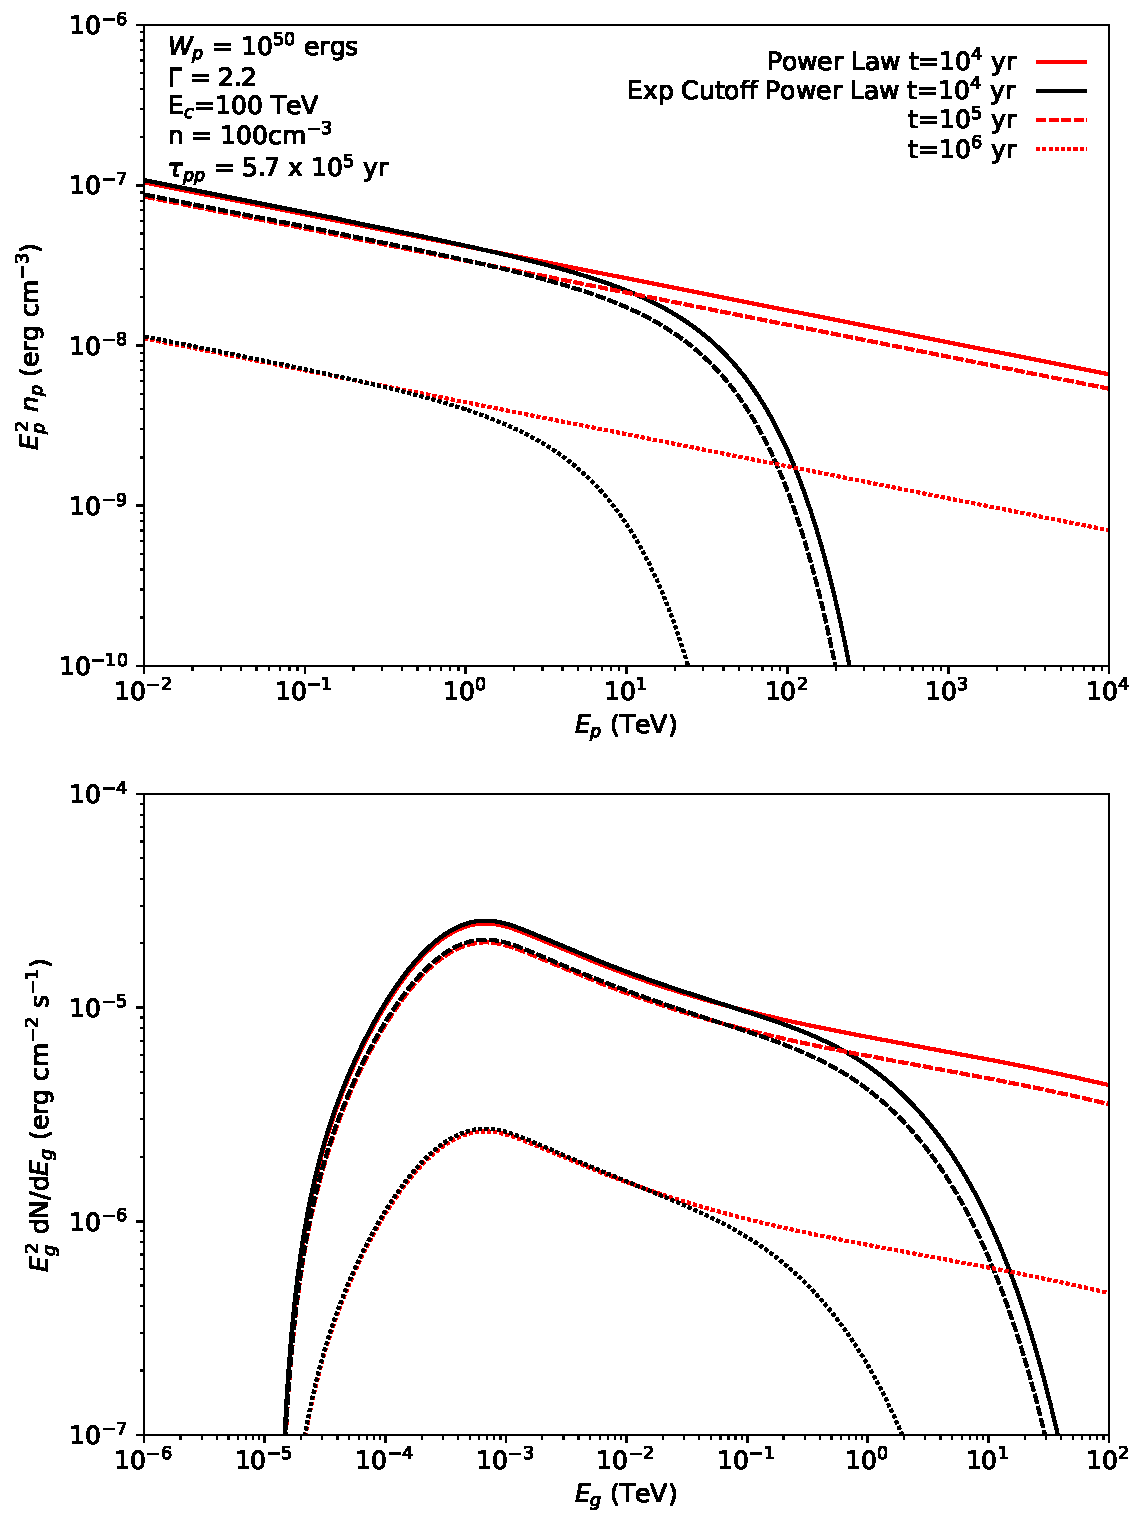
\includegraphics[width=1.0\textwidth]{07_Particle_Evolution/Images/evolution/impulsive_proton_total_spectrum.pdf}
	\caption{Evolution of the cosmic-ray energy density distribution (\textit{top}) and subsequent gamma-ray SED (\textit{bottom}) for an impulsive source injecting protons following a power law spectrum ($\propto E^{-\Gamma}$, red) and an exponential cutoff power law spectrum ($\propto E^{-\Gamma}\exp(-E/E_c)$, black) as given by \autoref{eq:chapter_7_imp_hadronic_cr_energy_distrib}. $W_p$ is the total energy of cosmic-ray protons injected at $t=0$.1q}
	\label{fig:chapter_7_impulsive_hadron_cr_spectrum}
\end{figure}

The top panel of \autoref{fig:chapter_7_impulsive_hadron_cr_spectrum} shows the evolution of a hadronic cosmic-ray energy density distribution and subsequent gamma-ray SED for an initial power law spectrum ($\Gamma=2.2$) and an exponential cutoff power law spectrum ($\Gamma=2.2$, $E_c=100~\TeV$). As the age of the system increases beyond the proton cooling time (i.e. $t>\tau_{pp}=5.3\times 10^5~\si{yr}$), the cosmic-ray density and subsequent gamma-ray emission decreases (see \autoref{sec:chapter1_hadronic_gr_emission}).

\subsubsection{Leptonic Cosmic-Ray Source}

Assuming synchrotron losses are dominant (valid for high-energy electrons and/or regions of high magnetic field strength, see \autoref{eq:chapter_1_non_thermal_leptonic_cooling_rate2}), the leptonic cooling rate is given by:

\begin{equation}
    \begin{aligned}
        \dot{\gamma}&=-b_s\gamma^2 \text{ ,}
    \end{aligned}\label{eq:chapter_7_lepton_loss_rate}
\end{equation}
\noindent where $b_s = 1.292 \times 10^{-15} \qty(B/\si{\milli G})^2~\si{\per\second}$ is the synchrotron loss term for electrons. The solution for \autoref{eq:chapter_7_lepton_loss_rate} is:

\begin{equation}
	\begin{aligned}
		\gamma_0&=\frac{\gamma}{1-\gamma b_s t} \text{ ,}
	\end{aligned} \label{eq:chapter_7_imp_leptonic_lorentz_initial}
\end{equation}
\noindent giving the initial electron distribution in terms of Lorentz factor $\gamma$:
\begin{equation}
    \begin{aligned}
        n_e\qty(\gamma_0,0)&=A\gamma^{-\Gamma}\qty(1-\gamma b_s t)^{\Gamma}\exp(-\frac{\gamma}{\gamma_c\qty(1-\gamma b_st)})\text{ .} 
    \end{aligned} \label{eq:chapter_7_imp_leptonic_cr_initial_distrib}
\end{equation}
\noindent From \autoref{eq:chapter_7_imp_leptonic_lorentz_initial} it can be seen that at any time, $t$, there exists a critical Lorentz factor:

\begin{equation}
    \begin{aligned}
    \gamma_\text{cr}&=\frac{1}{b_s t} \text{ ,}
    \end{aligned}\label{eq:chapter_7_imp_lep_critical_lorentz}
\end{equation}
\noindent where electrons with $\gamma_\text{cr}$ have an initial Lorentz factor, $\gamma_0\rightarrow \infty$. An impulsive system at time $t$ cannot have electrons exceeding this critical Lorentz factor.
\par
\noindent As $\dot{\gamma}_0=-b_s\gamma^2$:

\begin{equation}
	\begin{aligned}
		\frac{\dot{\gamma}_0}{\dot{\gamma}}&=\qty(\frac{\gamma_0}{\gamma})^2 \text{ ,}
	\end{aligned} \label{eq:chapter_7_gamma_gamma_0_ratio}
\end{equation}
\noindent \autoref{eq:chapter_7_cr_energy_distribution_imp} and \autoref{eq:chapter_7_imp_leptonic_cr_initial_distrib} can be combined to find the cosmic-ray energy density distribution for electrons with Lorentz factor $\gamma$:

\begin{equation}
    \begin{aligned}
    n_e\qty(\gamma,t)&=A\gamma^{-\Gamma}\qty(1-\gamma b_s t)^{\Gamma-2}\exp(-\frac{\gamma}{\gamma_c\qty(1-\gamma b_st)})\text{ .}
    \end{aligned} \label{eq:chapter_7_imp_leptonic_cr_energy_distrib}
\end{equation}
\begin{figure}[hbtp]
	\centering
	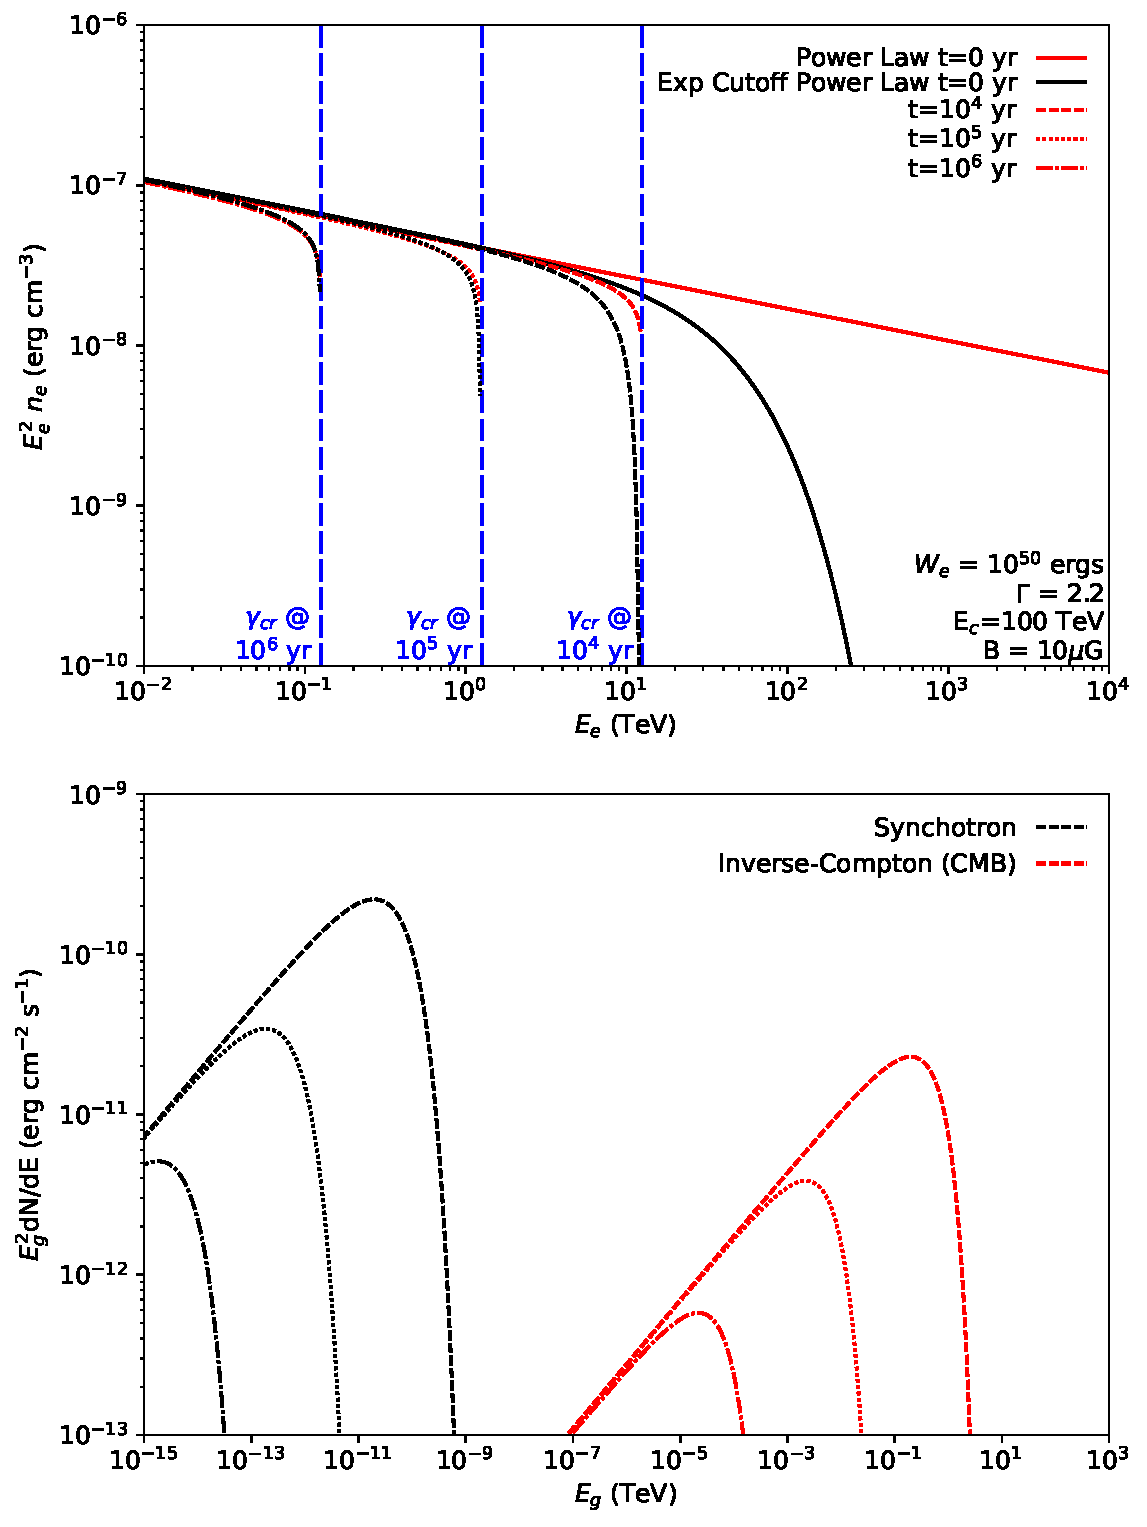
\includegraphics[width=1.0\textwidth]{07_Particle_Evolution/Images/evolution/impulsive_electron_total_spectrum.pdf}
	\caption{Evolution of the cosmic-ray energy density distribution (\textit{top}) and subsequent gamma-ray SED (\textit{bottom}) for an impulsive source injecting electrons following a power law spectrum (red) and an exponential cutoff power law spectrum (black) as given by \autoref{eq:chapter_7_imp_leptonic_cr_energy_distrib}. The critical Lorentz factor (\autoref{eq:chapter_7_imp_lep_critical_lorentz}) at different ages are shown by the vertical blue-dashed lines.}
	\label{fig:chapter_7_impulsive_lepton_cr_spectrum}
\end{figure}
\autoref{fig:chapter_7_impulsive_lepton_cr_spectrum} shows the energy density distribution evolution of electrons and the subsequent gamma-ray emission for an impulsive source with an initial power law and exponential cutoff power law spectrum. As the system ages, the critical Lorentz factor (see \autoref{eq:chapter_7_imp_lep_critical_lorentz}) decreases and the energy density distribution can be described by an exponential cutoff power regardless of the distribution at times, $t=0~\si{\year}$. The peak in the subsequent synchrotron and inverse Compton emission shifts to lower energies as the system evolves in time.


\subsection{Continuous Source of Cosmic Rays}

A continuous source is a source that injects cosmic rays into the ISM at a constant rate over a significant time frame. For simplicity, it's assumed that source has a constant injection luminosity; i.e. no outbursts or `dormant' stages. Examples of continuous sources include pulsars and massive stellar clusters which typically inject cosmic rays for over $10^5~\si{yr}$. At $t=0~\si{yr}$ the initial cosmic-ray density, $n\qty(\gamma_0,0)$, is zero. Assuming that no cosmic rays escape the system ($\lambda=0$), \autoref{eq:chapter_7_cr_energy_distribution_transform_sol} becomes:

\begin{equation}
    \begin{aligned}
    	n\qty(\gamma,t)&=\frac{1}{\dot{\gamma}\qty(\gamma)}\int_\gamma^{\gamma_0} S\qty(\gamma',t-\tau\qty(\gamma',\gamma))\dd{\gamma'} \text{ ,}
    \end{aligned} \label{eq:chapter_7_cr_energy_distribution_cont} 
\end{equation}
\noindent and it will be assumed that the electron energy distribution of accelerators such as PWNe follow a power law (e.g. \citep{2014JHEAp...1...31T}). Hence, the source term in \autoref{eq:chapter_7_cr_energy_distribution_cont} will follow:

\begin{equation}
    \begin{aligned}
    S\qty(\gamma,t)&=A\gamma^{-\Gamma} \text{ .}
    \end{aligned} \label{eq:chapter_7_cr_energy_distribution_cont_t0} 
\end{equation}

\subsubsection{Hadronic Cosmic-Ray Source}

Combining \autoref{eq:chaper_7_hadron_loss_rate}, \autoref{eq:chapter_7_hadron_loss_solution}, \autoref{eq:chapter_7_cr_energy_distribution_cont} \& \autoref{eq:chapter_7_cr_energy_distribution_cont_t0} gives the proton energy density distribution at Lorentz factor $\gamma$:

\begin{equation}
    \begin{aligned}
    n_p\qty(\gamma,t)&=\frac{A\tau_{pp}}{\gamma}\int_\gamma^{\gamma_0} \gamma^{-\Gamma} \dd{\gamma'} \\
	&=\frac{A\tau_{pp}}{\gamma(\Gamma-1)}\qty[\gamma^{1-\Gamma}-\gamma_0^{1-\Gamma}] \\
	&=\frac{A\tau_{pp}}{\gamma(\Gamma-1)}\qty[\gamma^{1-\Gamma}-\qty(\gamma\exp(t/\tau_{pp}))^{1-\Gamma}] \\
	&=\frac{A\tau_{pp}\gamma^{\Gamma}-1}{\gamma(\Gamma-1)}\qty[1-\exp(-\frac{t\qty(\Gamma-1)}{\tau_{pp}})] \\
	&=\frac{\tau_{pp}A\gamma^{-\Gamma}}{\Gamma-1}\qty[1-\exp(-\frac{t\qty(\Gamma-1)}{\tau_{pp}})] \text{ .}
    \end{aligned} \label{eq:chapter_7_cont_hadronic_cr_energy_distrib}
\end{equation}

At $t=0$, the cosmic-ray energy density distribution is initially zero. As the system ages ($t\gg\tau_{pp}$), a steady state occurs when the energy loss through p-p interactions is balanced by the energy injected by the source (see \autoref{fig:chapter_7_continuous_hadron_cr_spectrum}). The steady state ($t\gg \tau_{pp}$) has an energy spectrum:
\begin{equation}
    \begin{aligned}
    	n_p\qty(\gamma, t\gg \tau_{pp})&=\frac{\tau_{pp}A\gamma^{-\Gamma}}{1-\Gamma}\text{ .}
    \end{aligned} \label{eq:07_cont_hadronic_cr_steady_state}
\end{equation}
\begin{figure}[hbtp]
	\centering
	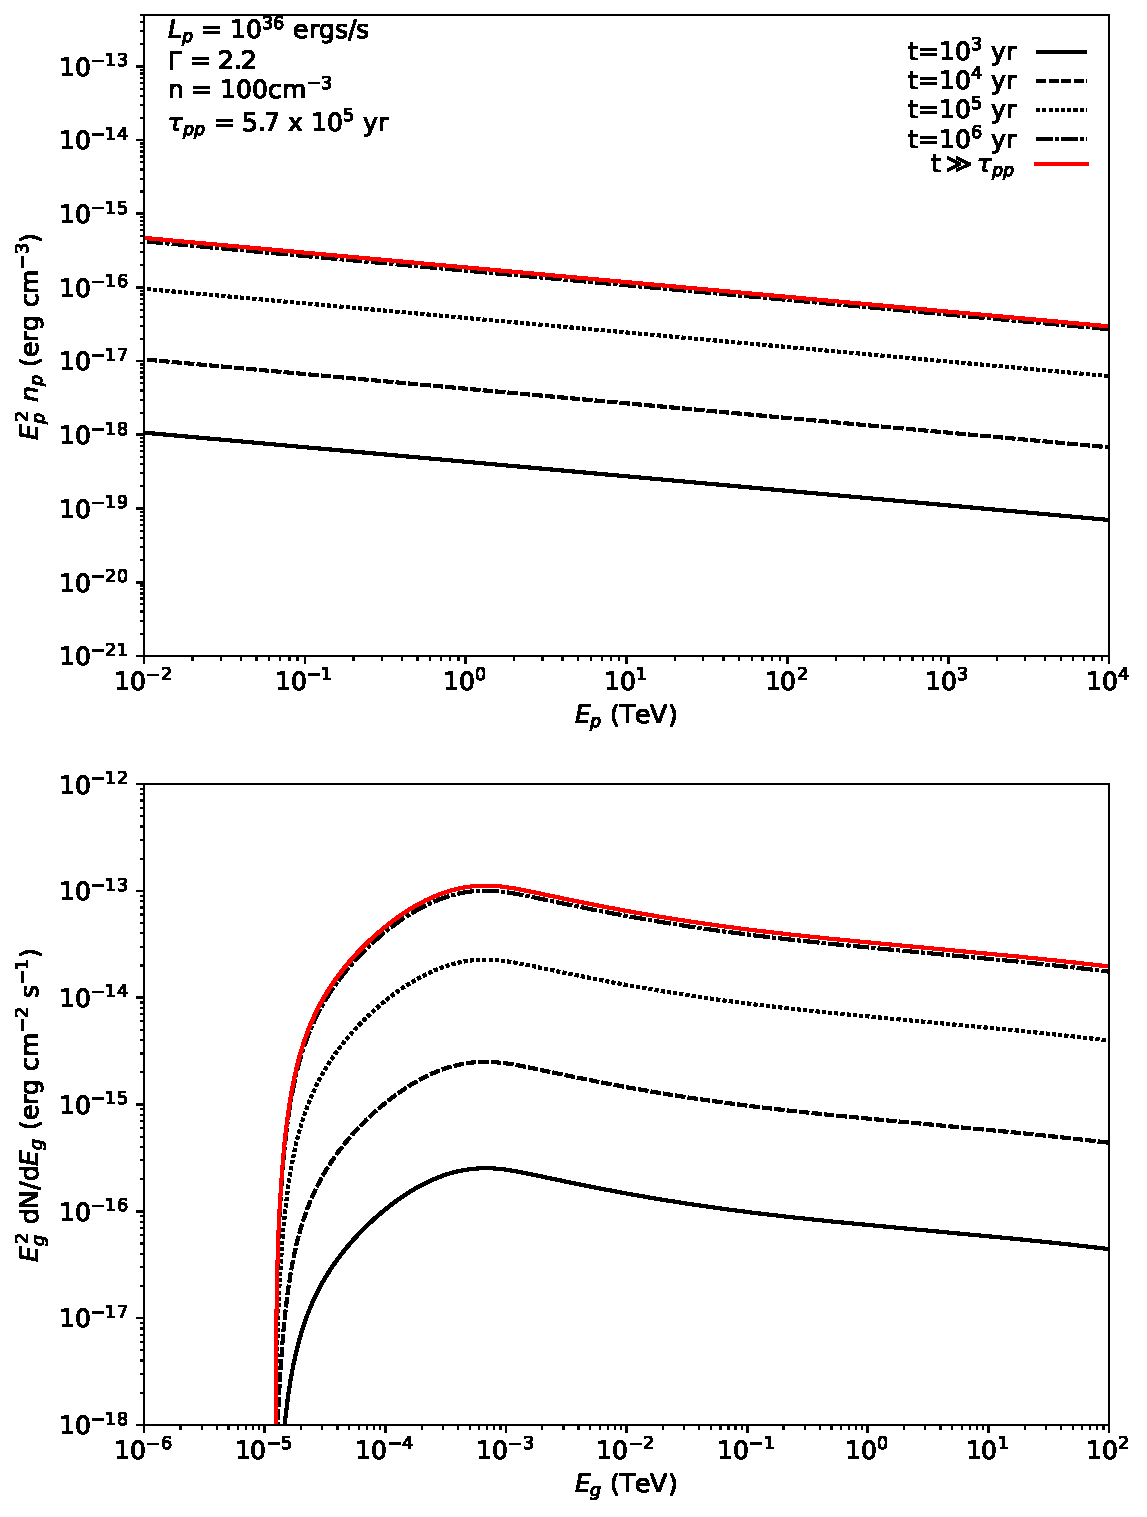
\includegraphics[width=1.0\textwidth]{07_Particle_Evolution/Images/evolution/continuous_proton_total_spectrum.pdf}
	\caption{Evolution of the cosmic-ray energy density distribution (top) and subsequent gamma-ray spectrum (bottom) for a continuous source injecting protons following a power law spectrum as given by \autoref{eq:chapter_7_cont_hadronic_cr_energy_distrib}. The steady state ($t\gg \tau_{pp}$, see \autoref{eq:07_cont_hadronic_cr_steady_state}) is represented by the solid red line. $L_p$ is the energy of cosmic rays injected per second into the system.}
	\label{fig:chapter_7_continuous_hadron_cr_spectrum}
\end{figure}
\autoref{fig:chapter_7_continuous_hadron_cr_spectrum} shows the evolution of the cosmic-ray and subsequent gamma-ray spectra for a system that continuously injects protons into a system with proton-proton cooling time of $5.7\times 10^5~\si{yr}$.

\subsubsection{Leptonic Cosmic-Ray Source}
Again, synchrotron radiation is assumed to be the dominant cause of electron energy loss. From \autoref{eq:chapter_7_imp_leptonic_lorentz_initial} \& \autoref{eq:chapter_7_imp_lep_critical_lorentz}, electrons with Lorentz factor greater than the critical Lorentz factor ($\gamma\geq\gamma_\text{cr}$) must be treated separately:

\begin{equation}
    \begin{aligned}
    	n_e\qty(\gamma)&=
	\begin{cases}
	\frac{1}{\dot{\gamma}\qty(\gamma)}\int_{\gamma}^{\gamma_0}S\qty(\gamma',t-\tau\qty(\gamma',\gamma))\dd{\gamma'}  &\gamma < \gamma_\text{cr}\\
	\frac{1}{\dot{\gamma}\qty(\gamma)}\int_{\gamma}^{\infty}S\qty(\gamma',t-\tau\qty(\gamma',\gamma))\dd{\gamma'} &\gamma \geq \gamma_\text{cr}\\
	\end{cases}\text{ .} \label{eq:chapter_7_cr_energy_dist_lept_cont_final}
    \end{aligned}
\end{equation}
\noindent For $\gamma < \gamma_\text{cr}$, combining \autoref{eq:chapter_7_lepton_loss_rate}, \autoref{eq:chapter_7_imp_leptonic_lorentz_initial}, \autoref{eq:chapter_7_cr_energy_distribution_cont_t0} \& \autoref{eq:chapter_7_cr_energy_dist_lept_cont_final}:

\begin{equation}
    \begin{aligned}
    	n_e\qty(\gamma< \gamma_\text{cr})&=\frac{A}{b_s\gamma^2\qty(\Gamma-1)}\qty[\gamma^{1-\Gamma}-\gamma_0^{1-\Gamma}] \\
	&=\frac{A}{b_s\gamma^2\qty(\Gamma-1)}\qty[\gamma^{1-\Gamma}-\frac{\gamma^{1-\Gamma}}{\qty(1-\gamma b_s t)^{1-\Gamma}}] \\
	&=\frac{A\gamma^{-\Gamma}\gamma}{b_s\gamma^2\qty(\Gamma-1)}\qty[1-\frac{1}{\qty(1-\gamma b_s t)^{1-\Gamma}}] \\
	&=\frac{A\gamma^{-\Gamma}}{b_s\gamma\qty(\Gamma-1)}\qty[1-\qty(1-\gamma b_s t)^{\Gamma-1}]\text{ .}
    \end{aligned}
\end{equation}
\noindent For $\gamma \geq \gamma_\text{cr}$:

\begin{equation}
    \begin{aligned}
    n_e\qty(\gamma\geq \gamma_\text{cr})&=\frac{A}{b_s\gamma^2\qty(1-\Gamma)}\qty(\infty^{1-\Gamma}-\gamma^{1-\Gamma}) \\
	&=\frac{A\gamma^{-\Gamma}}{b_s\gamma\qty(\Gamma-1)}\text{ .}
    \end{aligned}
\end{equation}
\noindent Therefore:

\begin{equation}
    \begin{aligned}
    n_e\qty(\gamma)&=\frac{A\gamma^{-\Gamma}}{b_s\gamma\qty(\Gamma-1)}
	\begin{cases}
		\qty[1-\qty(1-\gamma b_s t)^{\Gamma-1}] &\gamma < \gamma_\text{cr}\\
		1 &\gamma \geq \gamma_\text{cr}\\
	\end{cases} \text{ .}
    \end{aligned} \label{eq:chapter_7_cont_leptonic_cr_energy_distrib}
\end{equation}
\noindent A steady state is reached when:

\begin{equation}
    \begin{aligned}
        t\equiv\tau = (\gamma b_s)^{-1} = \tau_\text{sync}\text{ ,}
    \end{aligned} \label{eq:07_cont_leptonic_cr_steady_state}
\end{equation}
\begin{figure} [hbtp]
	\centering
	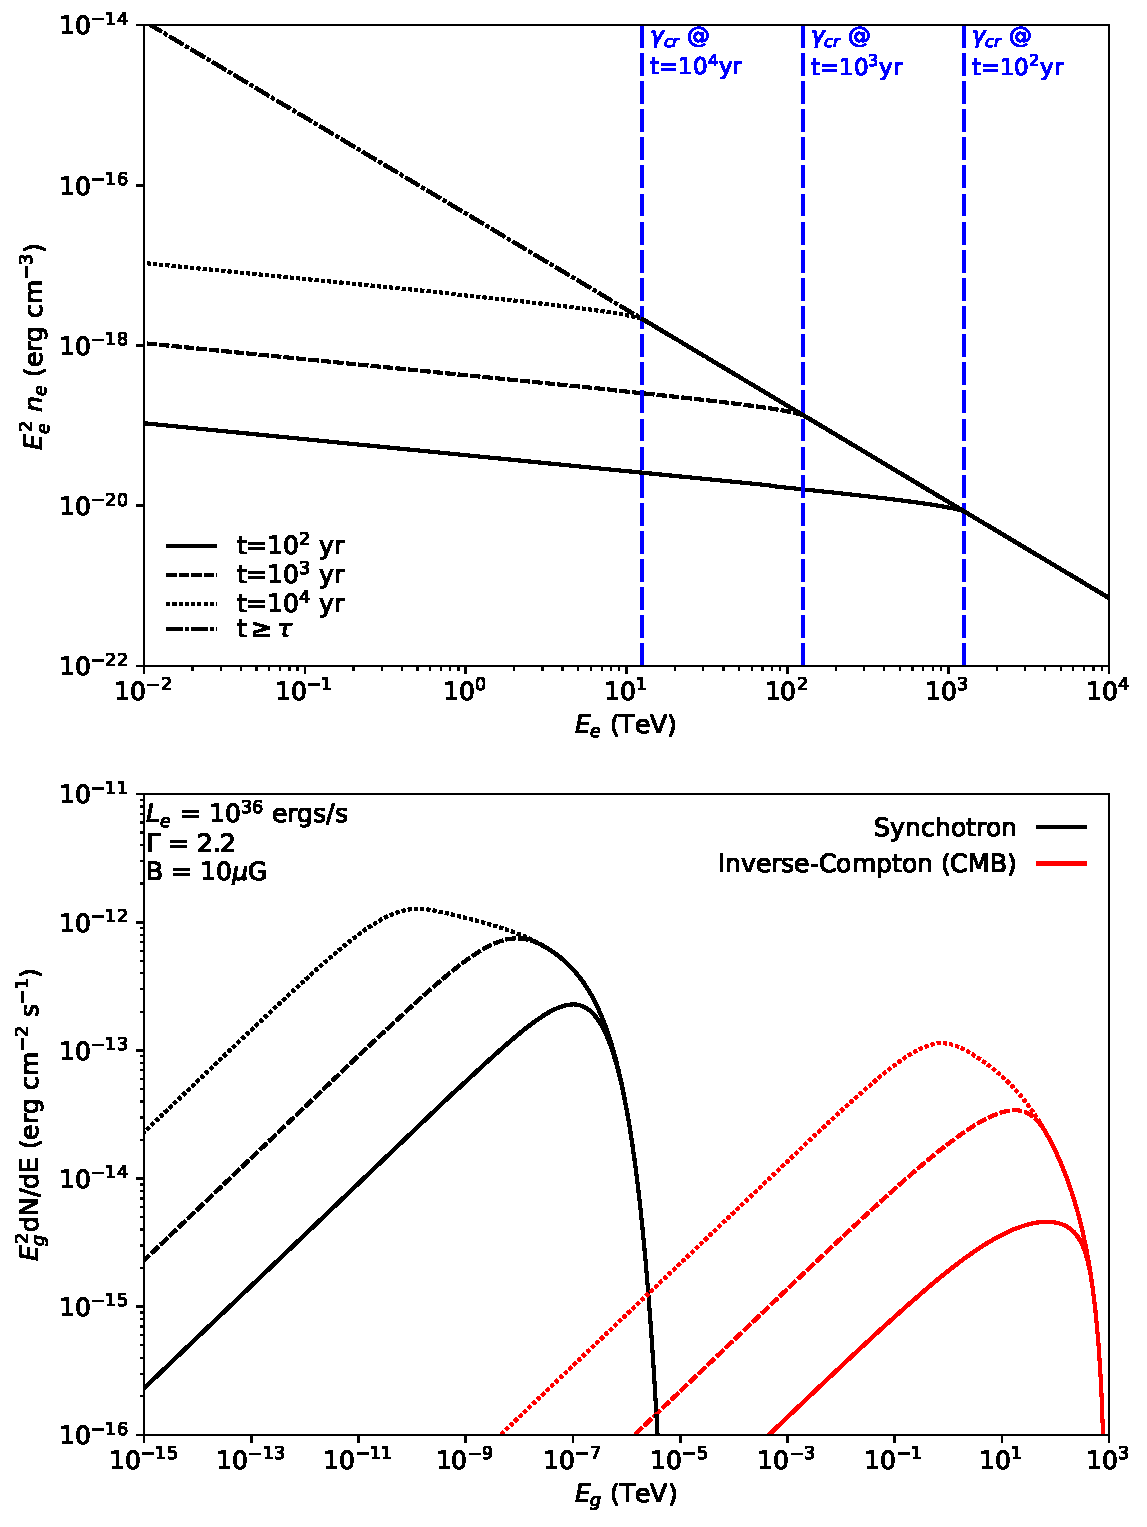
\includegraphics[width=1.0\textwidth]{07_Particle_Evolution/Images/evolution/continuous_electron_total_spectrum.pdf}
	\caption{Evolution of the cosmic-ray energy density distribution (\textit{top}) and subsequent gamma-ray SED (\textit{bottom}) for a continuous source injecting electrons following a power law spectrum as given by \autoref{eq:chapter_7_cont_leptonic_cr_energy_distrib}. The steady state of electrons ($t\gg \tau\approx \tau_\text{sync}$, see \autoref{eq:07_cont_leptonic_cr_steady_state}) is represented by the dash-dot line. $L_e$ is the energy of electrons injected per second into the system.}
	\label{fig:chapter_7_continuous_lepton_cr_spectrum}
\end{figure}

\noindent where $\tau_\text{sync}$ is the cooling time of electrons through synchrotron emission. The evolution of the electron spectra and subsequent gamma-ray spectra is shown in \autoref{fig:chapter_7_continuous_lepton_cr_spectrum}. Unlike protons, where the cooling time, $\tau_{pp}$, is dependent only on the medium's number density, the cooling time for electrons through synchrotron radiation is inversely proportional to their energy. Therefore, high-energy electrons reach a steady state before lower energy electrons.

\section{Transport of Cosmic Rays} \label{sec:chapter_7_cr_SED_trans} 

\autoref{eq:chapter_7_imp_hadronic_cr_energy_distrib}, \autoref{eq:chapter_7_imp_leptonic_cr_energy_distrib}, \autoref{eq:chapter_7_cont_hadronic_cr_energy_distrib} and \autoref{eq:chapter_7_cont_leptonic_cr_energy_distrib} describe the evolution of the spectral energy density distribution of cosmic rays at the location of the source. However, cosmic rays propagate from their place of birth into the ISM through diffusion (see \autoref{chapter_1_cr_propagation}). This section will describe how the cosmic-ray energy density distribution spatially and temporally evolves as a function of distance, $r$, from the accelerator.

\subsection{Propagation of Cosmic Rays}

We will take the simple example of an impulsive cosmic-ray source injecting particles with power law spectrum ($n\qty(\gamma,r=0,t=0)=A\gamma^{-\Gamma}$) into the centre of a uniform cloud at $t=0$. The cosmic rays are then allowed to propagate outwards. \cite{1995PhRvD..52.3265A} gives the Green's function solution of \autoref{eq:chapter_7_cr_energy_distribution_sol} at a distance $r$ from an impulsive source:

\begin{subequations}
	\begin{align}
	n\qty(\gamma,t,r)&=\frac{\dot{\gamma}_0}{\dot{\gamma}}\frac{n\qty(\gamma,0,0)}{\pi^{\frac{3}{2}}R_\text{diff}\qty(\gamma,t,B)^3}\exp\qty(-\frac{r^2}{R_\text{diff}\qty(\gamma,t,B)^2}) \label{eq:chapter_7_cr_ev_green_solution} \\
	R_\text{diff}\qty(\gamma,t,B)&=\sqrt{4\int_\gamma^{\gamma_0}\frac{D\qty(\gamma',B)}{\dot{\gamma}'}\dd{\gamma'}}\text{ ,} \label{eq:chapter_7_R_ev_green_solution}
	\end{align}
\end{subequations}  
\noindent where $R_\text{diff}\qty(\gamma,t)$ represents the distance of which cosmic rays with Lorentz factor $\gamma$ propagate after time $t$, i.e. `diffusion distance' and $D\qty(\gamma,B)$ represents the diffusion coefficient for cosmic rays in a magnetic field strength $B$ (see \autoref{eq:diffusion}).

\subsubsection{Hadronic Cosmic-Ray Source}

Combining \autoref{eq:chaper_7_hadron_loss_rate} and \autoref{eq:chapter_7_R_ev_green_solution} gives the evolution of the diffusion radius at distance $r$ from the accelerator:

\begin{equation}
	\begin{aligned}
		R_\text{diff}\qty(\gamma,t,B)&=\sqrt{4\tau_{pp}\chi D_0\qty(\frac{B}{3~\si{\micro G}})^{-\delta}\int_\gamma^{\gamma_0}\gamma'^{\delta-1}\dd{\gamma'}} \\
		&=\sqrt{4\tau_{pp}\chi D_0\qty(\frac{B}{3~\si{\micro G}})^{-\delta}\qty{\gamma_0^\delta-\gamma^\delta}} \\
		&=\sqrt{4\tau_{pp}\chi D_0\qty(\frac{B}{3~\si{\micro G}})^{-\delta}\qty{\gamma^\delta\exp\qty(\gamma t/\tau_{pp})-\gamma^\delta}} \\
		&=\sqrt{4D\qty(\gamma,B)t\frac{\qty(\exp(\frac{\delta t}{\tau_{pp}})-1)}{\delta t/\tau_{pp}}}\text{ .}
	\end{aligned} \label{eq:chapter_7_Rdiff_hadronic_impulsive}
\end{equation} 

The time evolution of the cosmic-ray density distribution can be found by combining \autoref{eq:chaper_7_hadron_loss_rate}, \autoref{eq:chapter_7_imp_hadronic_cr_initial_distrib} and \autoref{eq:chapter_7_cr_ev_green_solution}:

\begin{equation}
	\begin{aligned}
		n_p\qty(\gamma,t,r)&=\frac{A\gamma^{-\Gamma}}{\pi^{\frac{3}{2}}R_\text{diff}\qty(\gamma,t,B)^3}\exp\qty(-\frac{\qty(\Gamma-1)t}{\tau_{pp}}-\frac{r^2}{R_\text{diff}\qty(\gamma,t,B)^2})\text{ .}
	\end{aligned} \label{eq:chapter_7_crpropev_hadronic_impulsive}
\end{equation}
\begin{figure}[hbtp]
	\centering
	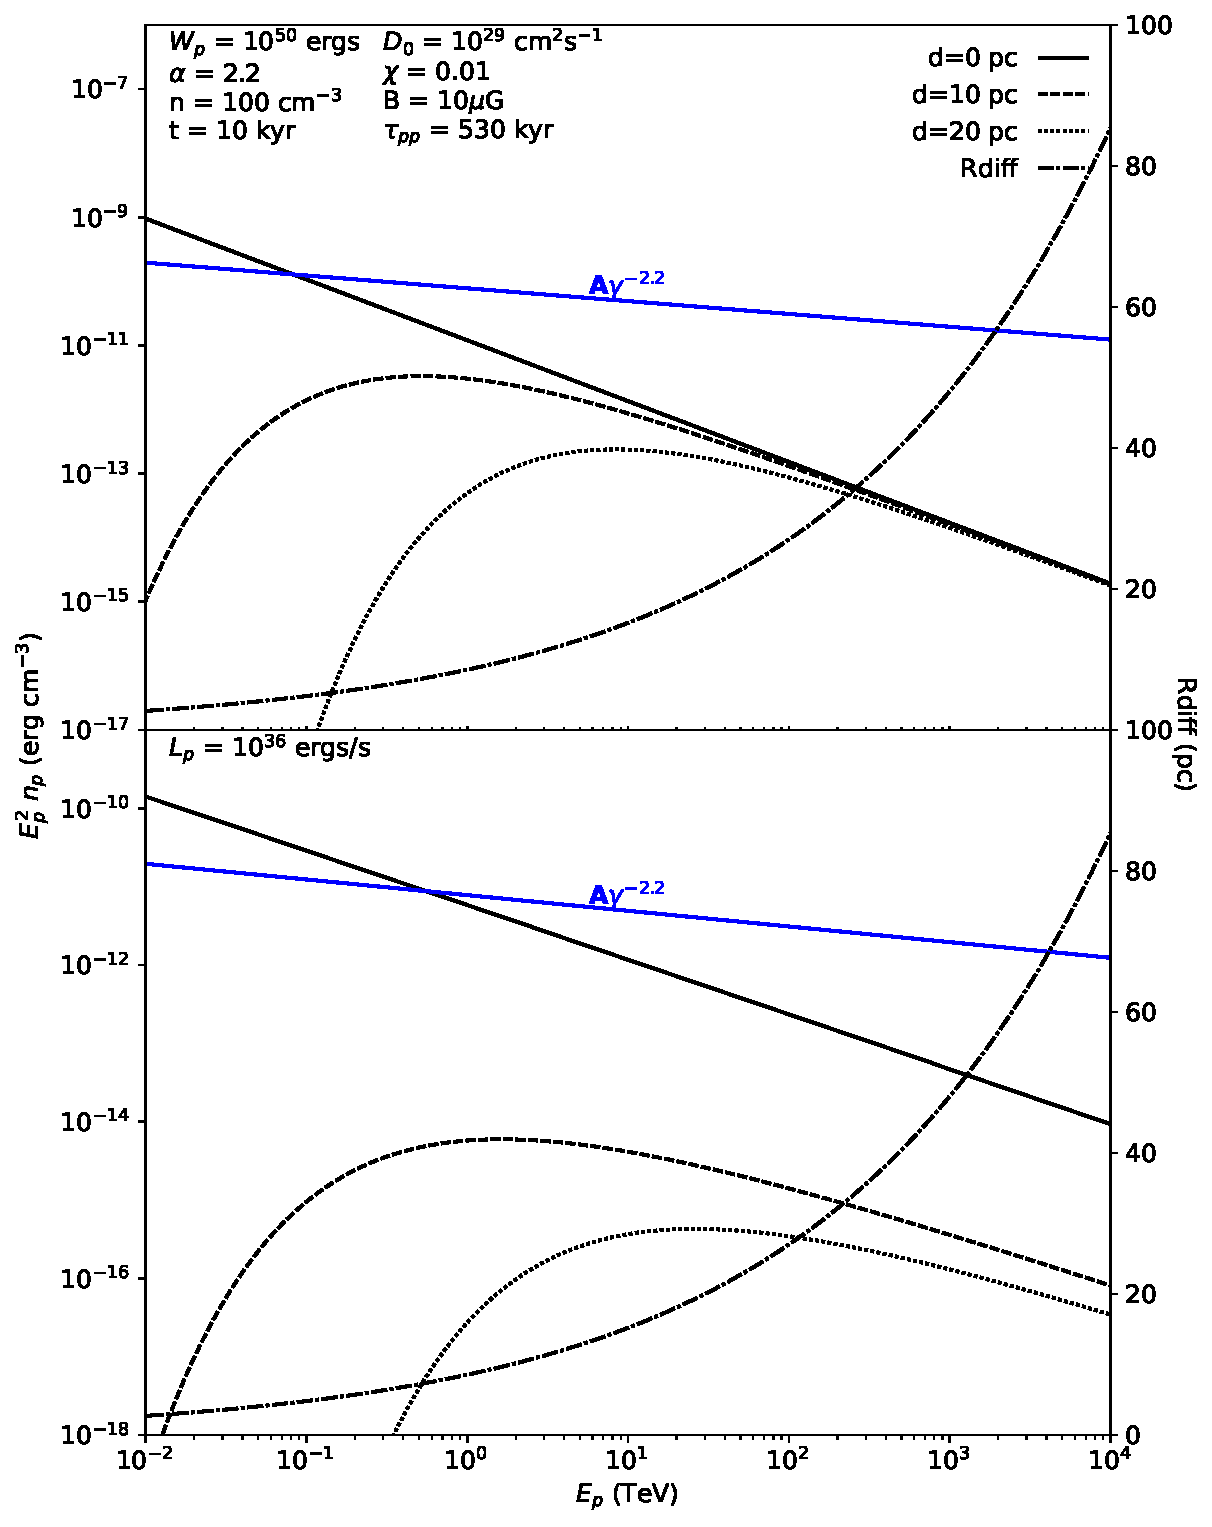
\includegraphics[width=\textwidth]{07_Particle_Evolution/Images/propagation/propagation_proton_cr_spectrum.pdf}
	\caption{The cosmic-ray energy density distribution for an impulsive (top panel) and continuous (bottom panel) source of protons after $10~\kiloyear$ as described by \autoref{eq:chapter_7_crpropev_hadronic_impulsive} and \autoref{eq:chapter_7_crpropev_hadronic_continuous} respectively. The solid blue line shows the shape of the injected proton energy distribution ($\propto E^{-\Gamma}$). For reference, the diffusion distance (\autoref{eq:chapter_7_Rdiff_hadronic_impulsive}) is represented by the dashed-dotted line.}
	\label{fig:chapter_7_propagation_hadron_cr_spectrum}
\end{figure}
\noindent The top panel of \autoref{fig:chapter_7_propagation_hadron_cr_spectrum} shows the hadronic cosmic-ray energy density distribution at different distances $r$ from an impulsive accelerator $10~\kiloyear$ after injecting cosmic rays with spectrum $n\qty(\gamma_0,0)=A\gamma^{-\Gamma}$ in a medium with number density and magnetic field $n=100~\si{\per\centi\meter\cubed}$ and $B=10~\si{\micro G}$ respectively. A diffusion suppression coefficient of $\chi=0.01$ was chosen to demonstrate the transport of cosmic rays in molecular clouds (see \autoref{chapter_1_cr_propagation}). \autoref{eq:chapter_7_Rdiff_hadronic_impulsive} and \autoref{fig:chapter_7_propagation_hadron_cr_spectrum} show that higher energy protons are able to diffuse further from the source than their lower energy counterparts. For distances far from the source, only the highest energy protons (e.g. $E\gtrapprox 30~\TeV$ for a distance of $20~\pc$) are able to reach this region for a given time. Hence, for distances greater than the diffusion length ($r>R_\text{diff}$), the proton energy spectra is steeper than the initial injected spectra. For distances close to the source, high-energy protons escape this region faster than low energy protons (e.g. a $1~\TeV$ and a $100~\TeV$ proton takes $\approx 14~\kiloyear$ and $\approx1.4~\kiloyear$ respectively to travel $5~\pc$). Therefore, for distances within the diffusion length ($r<R_\text{diff}$), the cosmic-energy density distribution is shallower than the injected spectrum. 
\par~\par
A continuous source can be treated as a series of impulsive injectors and \autoref{eq:chapter_7_cr_energy_distribution_sol} must be solved numerically. However, for a case when $t\ll \tau_{pp}$, the cosmic-ray energy density distribution can be described by \citep{1996A&A...309..917A}:

\begin{equation}
    \begin{aligned}
    n_p\qty(E,t,r)&=\frac{AE^{-\Gamma}}{4\pi D\qty(E,B)r}\text{erfc}\qty(\frac{r}{R_\text{diff}\qty(\gamma,t,B)}) \\
    \text{erfc}\qty(z)&=\frac{2}{\sqrt{\pi}}\int_z^\infty \exp(-x^2)\dd{x}\text{ .}
    \end{aligned} \label{eq:chapter_7_crpropev_hadronic_continuous}
\end{equation}
\noindent The bottom panel of \autoref{fig:chapter_7_propagation_hadron_cr_spectrum} shows the cosmic-ray energy density distribution at different distances $r$ from a continuous accelerator of protons. For distances close to the source ($R\ll R_\text{diff}$), the cosmic-ray energy spectrum is simply:
\begin{equation}
    \begin{aligned}
 	   n_p\qty(E,t,r)&=\frac{AE^{-\Gamma}}{4\pi D\qty(E,B)r}\text{ .}
    \end{aligned} 
\end{equation}
\noindent As $D\propto \gamma^{\delta}$ (see \autoref{eq:diffusion}), the cosmic-ray energy spectrum can be described by a power law with index $\Gamma+\delta$. The higher index (compared to the injected spectrum) mathematically describes high-energy cosmic rays escaping at a faster rate compared to low energy protons.

\subsubsection{Leptonic Cosmic-Ray Source}

For an accelerator injecting electrons, combining \autoref{eq:diffusion},  \autoref{eq:chapter_7_lepton_loss_rate} and \autoref{eq:chapter_7_R_ev_green_solution} gives the diffusion radius for electrons:

\begin{equation}
	\begin{aligned}
		R_\text{diff}\qty(\gamma,t,B)&=\sqrt{4b_s^{-1} \chi D_0\qty(\frac{B}{3~\si{\micro G}})^{-\delta}\int_\gamma^{\gamma_0}\gamma'^{\delta-2}\dd{\gamma'}} \\
		&=\sqrt{\frac{4}{b_s(\delta-1)} \chi D_0\qty(\frac{B}{3~\si{\micro G}})^{-\delta} \qty{\gamma_0^{\delta-1}-\gamma^{\delta-1}} } \\
		&=\sqrt{\frac{4}{b_s(\delta-1)} \chi D_0\qty(\frac{B}{3~\si{\micro G}})^{-\delta} \qty{\gamma^{\delta-1}\qty(1-\gamma b_st)^{\delta-1}-\gamma^{\delta-1}} } \\
		&=\sqrt{\frac{4D\qty(\gamma,B)}{b_s\gamma\qty(1-\delta)}\qty[1-\qty(1-\gamma b_s t)^{1-\delta}]}\text{ .}
	\end{aligned} \label{eq:chapter_7_Rdiff_leptonic_impulsive}
\end{equation} 
\noindent The leptonic energy density distribution for an impulsive injector is found by combining \autoref{eq:chapter_7_lepton_loss_rate}, \autoref{eq:chapter_7_cr_ev_green_solution} and \autoref{eq:chapter_7_imp_leptonic_cr_initial_distrib}:

\begin{equation}
	\begin{aligned}
		n_e\qty(\gamma,t,r)&=\frac{\qty(1-\gamma b_st)^{\Gamma-2}n_0\gamma^{-\Gamma}}{\pi^{\frac{3}{2}}R_\text{diff}\qty(\gamma,t,B)^3}\exp\qty(-\frac{r^2}{R_\text{diff}\qty(\gamma,t,B)^2})\text{ .}
	\end{aligned} \label{eq:chapter_7_crpropev_leptonic_impulsive}
\end{equation}
\begin{figure}[hbtp]
	\centering
	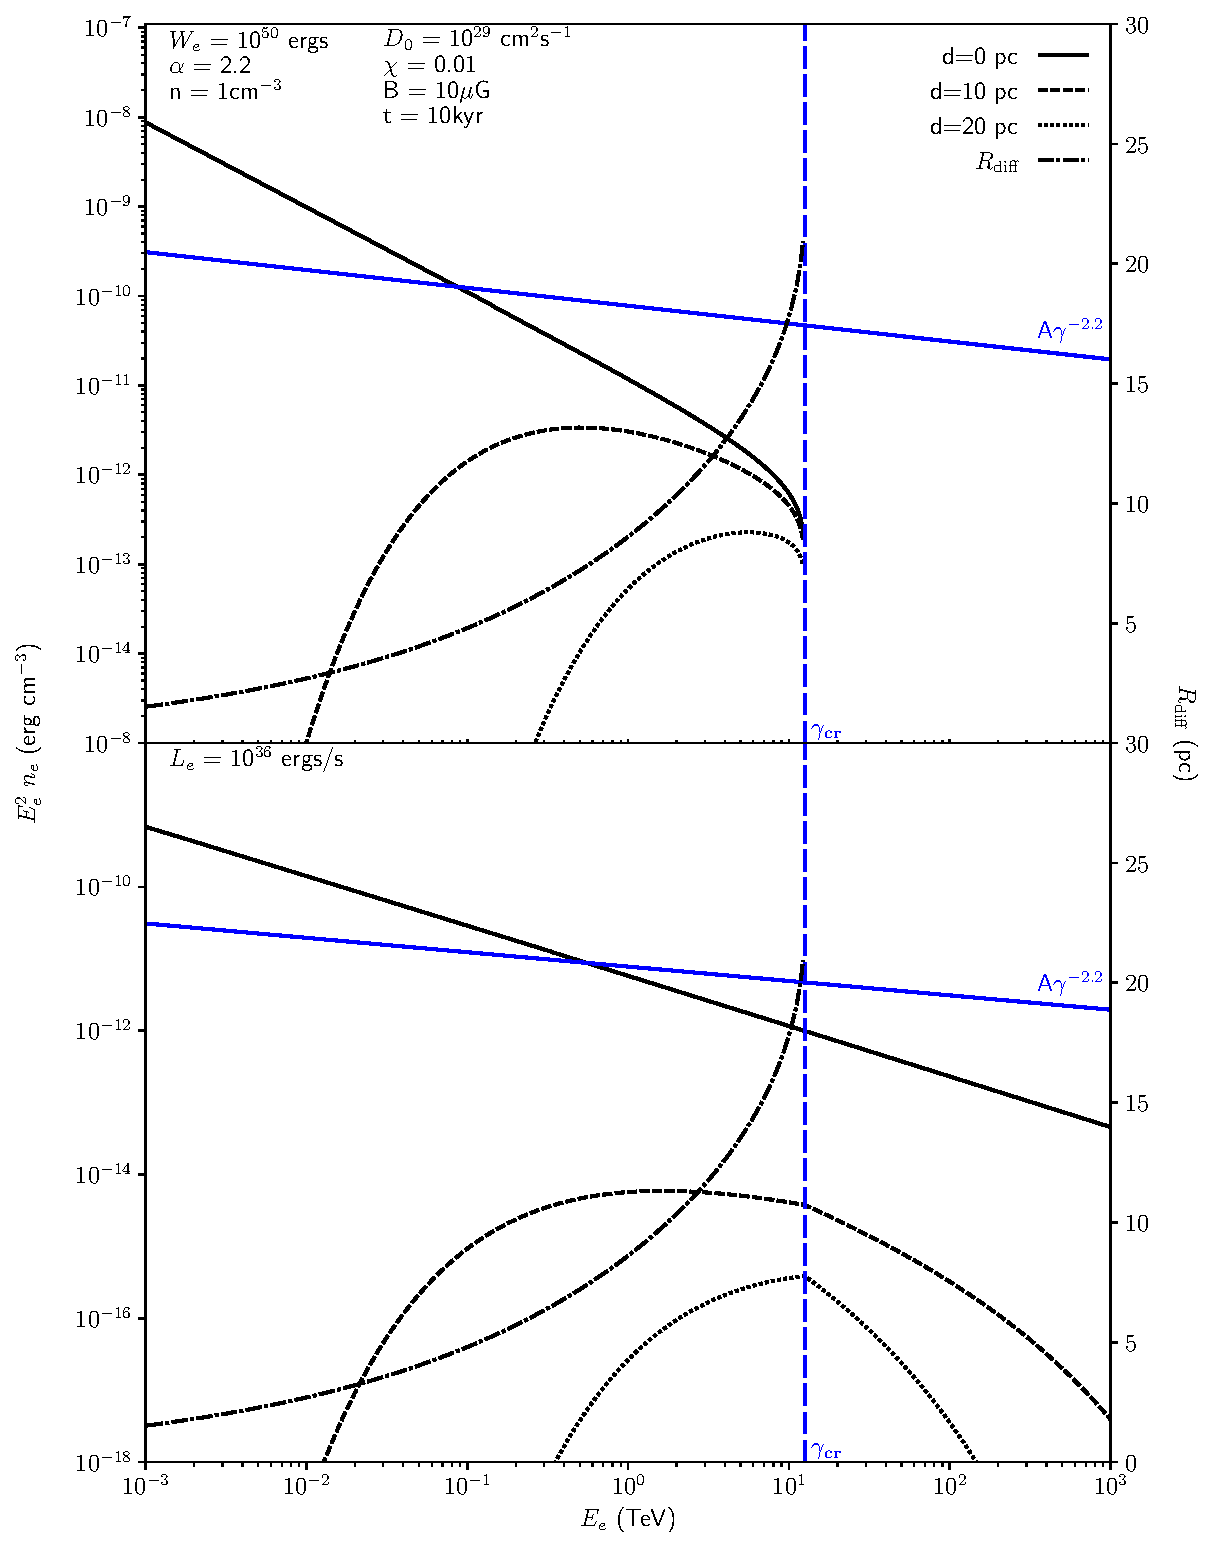
\includegraphics[width=1.0\textwidth]{07_Particle_Evolution/Images/propagation/propagation_electron_cr_spectrum.pdf}
	\caption{The cosmic-ray energy density distribution for an impulsive source (\textit{top}) and continuous source (\textit{bottom}) of electrons following a power law (solid blue line) after $t=10~\si{\kilo\year}$ as described by \autoref{eq:chapter_7_crpropev_leptonic_impulsive} and \autoref{eq:chapter_7_crpropev_leptonic_continuous} respectively. For reference, the diffusion distance is represented by the dashed-dotted line and the critical energy ($\gamma_{cr}\approx 13~\TeV$) is shown by the blue vertical dashed line.}
	\label{fig:chapter_7_propagation_leptonic_cr_spectrum}
\end{figure}
The top panel of \autoref{fig:chapter_7_propagation_leptonic_cr_spectrum} describes the leptonic energy density distribution at a distance $r$ from an impulsive injector $10~\kiloyear$ after injecting electrons with power law spectrum, $n\qty(\gamma,r=0,t=0)=A\gamma^{-\Gamma}$, into a medium with number density $1~\si{\per\centi\meter\cubed}$ and magnetic field $B=10~\si{\micro G}$. As with protons, high-energy electrons are able to diffuse to further than lower energy electrons. Therefore, for distances greater than the diffusion length ($r>R_\text{diff}$), the electron energy spectra is steeper than the injected spectra. For distances close to the source ($r<R_\text{diff}$), the electron energy spectra is shallower than the injected spectra. Unlike protons, a maximum electron energy can be seen corresponding to the critical Lorentz factor described by \autoref{eq:chapter_7_imp_lep_critical_lorentz}.
\par~\par
For a continuous source of electrons, \autoref{eq:chapter_7_cr_energy_distribution_sol} must be solved numerically. However, for a source injecting electrons constantly with a simple power law (and assuming synchrotron losses are dominant), \cite{1995PhRvD..52.3265A} gives the electron energy spectrum as:

\begin{equation}
    \begin{aligned}
    n_e\qty(E,t,r)&=\frac{n_0E^{-\Gamma}}{4\pi D\qty(E,B)r}\text{erfc}\qty(\frac{r}{2\sqrt{D\qty(E,B)t_\gamma}}) \\
    t_\gamma&=\text{min}\qty(t,\frac{1}{b_s\gamma})\text{ .}
    \end{aligned} \label{eq:chapter_7_crpropev_leptonic_continuous}
\end{equation}

Similarly to protons, for distances close to the source ($R\ll R_\text{diff}$), the electron energy spectrum is:
\begin{equation}
    \begin{aligned}
	    n_e\qty(E,t,r)&=\frac{AE^{-\Gamma}}{4\pi D\qty(E,B)r}\text{ ,}
    \end{aligned} 
\end{equation}

\noindent where $n_e\propto \gamma^{-\qty(\Gamma+\delta)}$.

\section{Modelling the Energy Density Distribution of Cosmic Rays}

\autoref{sec:chapter_7_cr_SED_evol} and \autoref{sec:chapter_7_cr_SED_trans} assumed simple scenarios in order to solve \autoref{eq:chapter_7_cr_energy_distribution_sol}. Such scenarios included the type of accelerator (impulsive or continuous) and whether the time of interest is less than the cooling time of the particle (e.g. \autoref{eq:chapter_7_crpropev_hadronic_continuous} and \autoref{eq:chapter_7_crpropev_leptonic_continuous}). It was also assumed that no particles escape the system (i.e. $v_\text{esc}=0$ in \autoref{eq:chapter_7_cr_energy_distribution}. For scenarios that do not make these assumptions, \autoref{eq:chapter_7_cr_energy_distribution_sol} must be solved analytically. A Reimann sum can be used to approximate the integral in \autoref{eq:chapter_7_cr_energy_distribution_sol} with:

\begin{equation}
    \begin{aligned}
	    n\qty(\gamma,t)&=\frac{1}{\dot{\gamma}\qty(\gamma)}\sum_{\gamma'=\gamma}^{\gamma_0} 	e^{-\lambda\qty(\gamma',\gamma)}S\qty(\gamma')\Delta \gamma' + 	\frac{\dot{\gamma_0}}{\dot{\gamma}}n\qty(\gamma_0,0)e^{-\lambda\qty(\gamma_0,\gamma)} 
    \end{aligned} \label{eq:chapter_7_single_zone_numerical}\text{ ,}
\end{equation}
\noindent where $\sum_{\gamma'=\gamma}^{\gamma_0}$ sums the function $e^{-\lambda\qty(\gamma',\gamma)}S\qty(\gamma')$ over Lorentz factor $\gamma'=\gamma\rightarrow \gamma_0$ in intervals of width $\Delta \gamma'$. The radiation loss rate, $\dot{\gamma}$, for cosmic-ray protons and electrons is calculated via \autoref{eq:chapter_1_pp_cooling time} and \autoref{eq:chapter_1_non_thermal_leptonic_cooling_rate2} respectively. This section will describe the software {\tt Newsedprod} which analytically solves \autoref{eq:chapter_7_cr_energy_distribution_sol}.

\subsection{{\tt Newsedprod}} \label{sec_chapter_7_newsedprod}

\begin{figure}[hbtp]
    \centering
    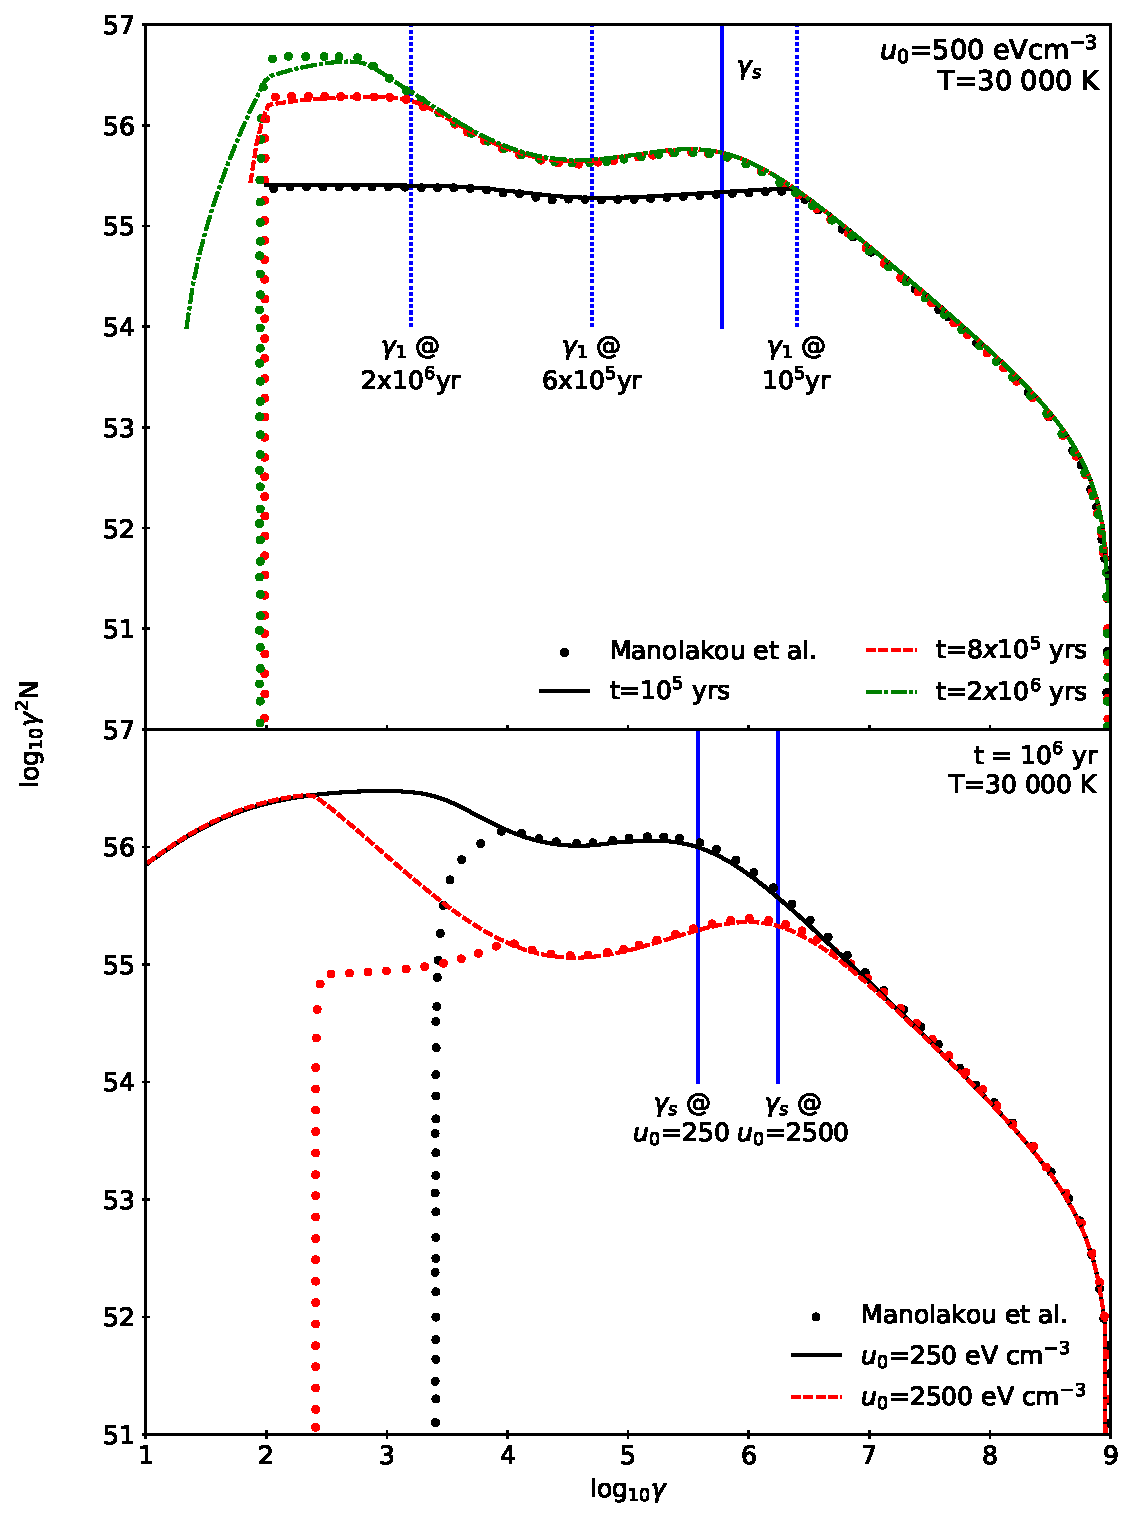
\includegraphics[width=\textwidth]{07_Particle_Evolution/Images/Code/manolakou_verification.pdf}
    \caption{Comparison of {\tt Newsedprod} (solid lines) and results by \cite{2007A&A...474..689M} (dots) where electrons between Lorentz factors $\gamma_\text{min}=10^2$ and $\gamma_\text{max}=10^9$ are injected with power law spectrum ($\Gamma =2.0$) into a medium with number density and magnetic field $n=1~\si{\per\centi\meter\cubed}$ and $B=10~\si{\micro G}$ respectively. Electrons are not allowed to escape the cloud ($\nu_\text{esc}=0$). (\textit{top}) Time evolution of electrons against a soft photon field of temperature $T=30000~\si{\kelvin}$ and energy density $u_0=500~\si{\electronvolt\per\centi\meter\cubed}$.  The positions of $\gamma_1$ (see \autoref{eq:chapter_7_gamma1_gamma2}) are shown by the solid vertical blue lines. (\textit{bottom}) The age of the system is kept constant at $10^6~\si{yr}$ while the energy density of the photon field is allowed to vary. Note that the variation at lower Lorentz factors is due to different values of $\gamma_\text{min}$ chosen by \cite{2007A&A...474..689M}.}
    \label{fig:chapter_7_manolakou_verification}
\end{figure}

{\tt Newsedprod} is a software originally developed by \citep{fabien} that injects cosmic rays into a uniform region of ISM (constant number density and magnetic field) with injection luminosity $W~\qty[\si{ergs\per\second}]$ (continuous source) or energy budget $L~\qty[\ergs]$  (impulsive source). The energy spectrum of cosmic-ray protons and electrons can be desribed by:

\begin{equation}
    \begin{aligned}
  	  J\qty(E)&= N_0 J'\qty(E)\quad\qty[\si{\per\tera\electronvolt\per\centi\meter\cubed}]\text{ ,}
    \end{aligned}
\end{equation}
\noindent where $N_0$ is the normalisation constant and $J'\qty(E)$ is the `denormalised' energy spectrum. The denormalised energy spectrum follows either:

\begin{itemize}
    \itemsep0em 
    \item power-law, $J'\qty(E)=E^{-\Gamma}$
    \item exponential cutoff power-law, $J'\qty(E)=E^{-\Gamma}\exp(-E/E_c)$, where $E_c$ is the cutoff energy
    \item broken power-law, $J'\qty(E)=(E/E_\text{break})^{-\Gamma_i}$, where $\Gamma_i=\Gamma_1$ for $E\leq E_\text{break}$ and $\Gamma_i = \Gamma_2$ otherwise
\end{itemize}

\noindent For an accelerator injecting cosmic rays (protons or electrons) with Lorentz factor between $\gamma_\text{min}$ and $\gamma_\text{max}$, the total amount of energy injected into the system must equate to the injection luminosity/energy budget:

\begin{equation}
    \begin{aligned}
 	   N_0&=\frac{L\text{ or }W\Delta t}{\int_{\gamma_\text{min}}^{\gamma_\text{max}} EJ'\qty(E)\dd{E}}\text{ ,}
    \end{aligned} \label{eq:chapter_7_energy_budget}
\end{equation}
\noindent where $W\Delta t$ represents the total energy injected into the system in time interval $\Delta t$.
\par~\par
After injection, cosmic rays radiate their energy and cool to lower Lorentz factors as described in \autoref{sec:chapter1_non_thermal_emission}. $\gamma_1$ and $\gamma_2$ are defined to be the Lorentz factors at time $t$ that correspond to the minimum, $\gamma_\text{min}$, and maximum, $\gamma_\text{max}$, Lorentz factor at $t=0$ before cooling:

\begin{equation}
    \begin{aligned}
    \tau\qty(\gamma_\text{max},\gamma_1) = t \\
    \tau\qty(\gamma_\text{min}, \gamma_2) = t\text{ ,}
    \end{aligned} \label{eq:chapter_7_gamma1_gamma2}
\end{equation}

\noindent where $\tau$ is the cooling time described in \autoref{eq:chapter_7_cooling_time}. Electrons with Lorentz factor $\gamma<\gamma_1$ represent the `uncooled' part of the spectrum and the energy density distribution follows the initial injected electron spectra ($\Gamma=2.0$). Electrons above $\gamma_1$ have reached a steady state where radiative losses are balanced by the injected electrons. To reduce computation time, \autoref{eq:chapter_7_single_zone_numerical} can be split into three different regimes:

\begin{equation}
    \begin{aligned}
    n\qty(\gamma,t)&=\frac{1}{\dot{\gamma}\qty(\gamma)}\sum_{\gamma'=\gamma_\ell}^{\gamma_u} e^{-\lambda\qty(\gamma',\gamma)}S\qty(\gamma')\Delta \gamma'\text{ ,}
    \end{aligned}  \label{eq:chapter_7_single_zone_numerical_manolakou}
\end{equation}

\noindent where $\gamma_\ell$ and $\gamma_u$ are the lower and upper Lorentz factors given by:

\begin{equation}
    \begin{aligned}
  	  \qty(\gamma_\ell,\gamma_u)&=
  	  \begin{cases}
  		  \qty(\gamma_\text{min},\gamma_0)\text{,}\quad & \gamma_2<\gamma\leq\gamma_\text{min} \\
  		  \qty(\gamma,\gamma_0)\text{,}\quad & \gamma_\text{min}<\gamma\leq\gamma_1 \\
		    \qty(\gamma,\gamma_\text{max})\text{,}\quad & \gamma_1<\gamma\leq\gamma_\text{max}
   	 \end{cases}\text{ ,}
    \end{aligned}
\end{equation}
\noindent for $\gamma_\text{min}<\gamma_1$ and:

\begin{equation}
    \begin{aligned}
  	  \qty(\gamma_\ell,\gamma_u)&=
  	  \begin{cases}
  		  \qty(\gamma_\text{min},\gamma_0)\text{,}\quad & \gamma_2<\gamma\leq\gamma_1 \\
   		 \qty(\gamma_\text{min},\gamma_\text{max})\text{,}\quad & \gamma_1<\gamma\leq\gamma_\text{min} \\
   		 \qty(\gamma,\gamma_\text{max})\text{,}\quad & \gamma_\text{min}<\gamma\leq\gamma_\text{max}
    	\end{cases}\text{ ,}
    \end{aligned}
\end{equation}
\noindent for $\gamma_\text{min}>\gamma_1$.
\par~\par
\autoref{fig:chapter_7_manolakou_verification} shows the comparison of the electron energy density distribution predicted by {\tt Newsedprod} to the results published by \cite{2007A&A...474..689M}. Assuming that there is no escape, i.e. ($\nu_\text{esc}=0$), electrons are continuously injected with an exponential cutoff power law spectrum ($\Gamma^{2.0}$) into a uniform cloud with number density $n=1~\si{\per\centi\meter\cubed}$ and magnetic field $B=10~\si{\micro G}$. The top panel of \autoref{fig:chapter_7_manolakou_verification} shows the time evolution of electrons against a soft photon field with temperature and energy density $T=30000~\si{K}$ and $u_0=500~\si{\electronvolt\per\centi\meter\cubed}$ (in line with the parameters chosen by \cite{2007A&A...474..689M}) at times $10^5~\si{yr}$ ($\gamma_1=2.5\times 10^6$), $8\times 10^5~\si{yr}$ ($\gamma_1=5\times 10^4$), $2\times 10^6~\si{yr}$ ($\gamma_1=1.6\times 10^3$). Synchrotron losses are dominant for electrons with Lorentz factor $\gamma>\gamma_s = 6\times 10^5$ (see \autoref{sec:chapter1_non_thermal_emission}). The bottom panel of \autoref{fig:chapter_7_manolakou_verification} investigates how the change in the photon field energy density affects the electron energy density distribution at time $10^6~\si{yr}$. Synchrotron losses are dominant for $\gamma>\gamma_s=3.8\times 10^5$ ($u_0=250~\si{\electronvolt\per\centi\meter\cubed}$) and $\gamma>\gamma_s=1.8\times 10^6$ ($u_0=2500~\si{\electronvolt\per\centi\meter\cubed}$).  \cite{2007A&A...474..689M} injects electrons between $\gamma_\text{min}=10^4$ and $\gamma_\text{min}=10^9$ while {\tt Newsedprod} injects electrons between $\gamma_\text{min}=10^{-2}$ and $\gamma_\text{min}=10^9$. The threshold Lorentz factor seen in the \cite{2007A&A...474..689M} corresponds to $\gamma=10^4$ at $t=0$ after being cooled, i.e. $\gamma_1$.

\par~\par
\begin{figure}[hbtp]
    \centering
    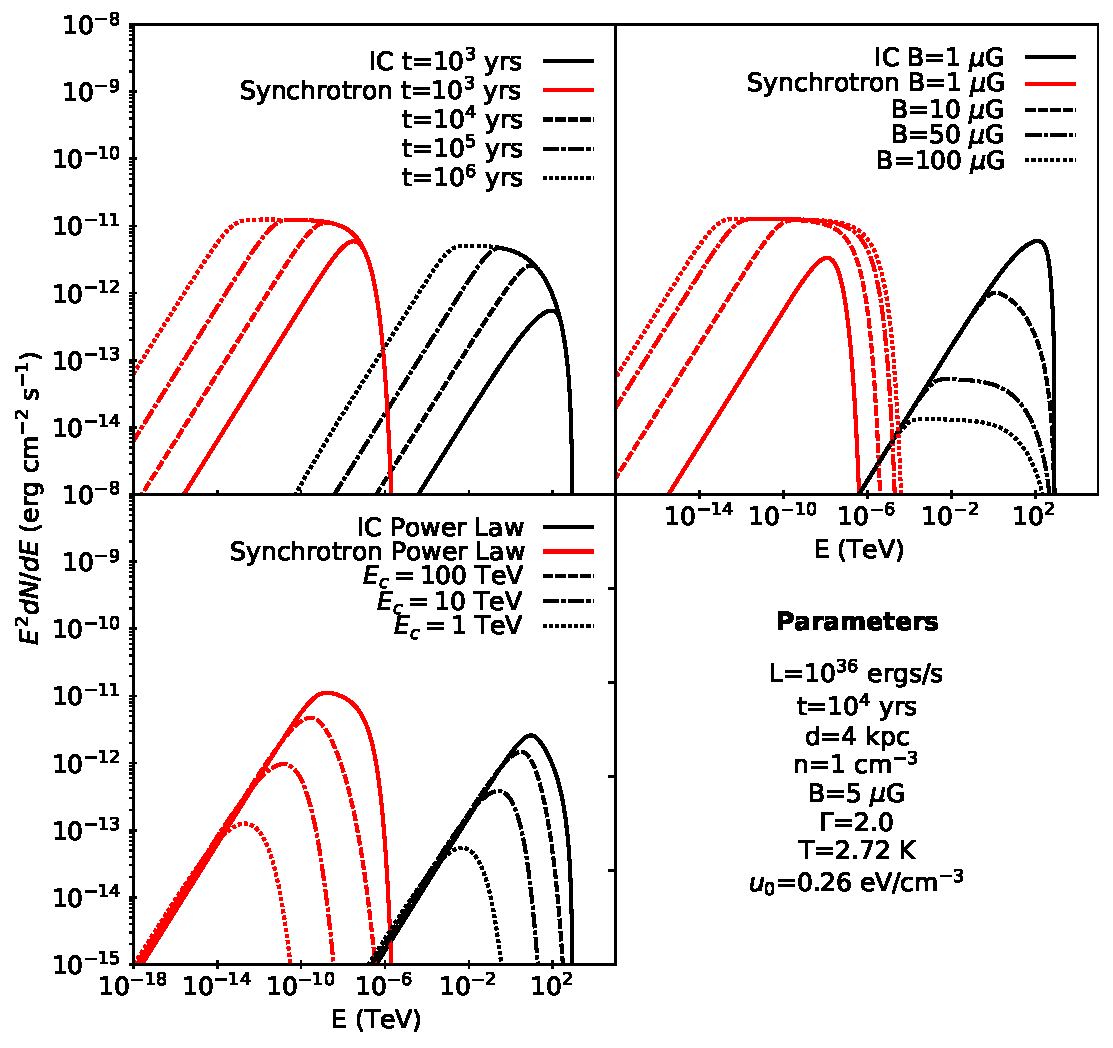
\includegraphics[width=\textwidth]{07_Particle_Evolution/Images/Code/leptonic_changing_variabls.pdf}
    \caption{The multiwavelength SED results from {\tt Newsedprod} for different scenarios of a continuous source. Unless otherwise stated, the input parameters are shown in the bottom-right panel ($L=$energy injection luminosity, $t=$age of system, $d=$distance to the cloud from Earth, $n=$density of ISM, $B=$background magnetic field, $\Gamma=$spectra of injected electrons, T and $u_0$ are the temperature and energy density of the background CMB field.)}
    \label{fig:chapter_7_newsedprod_leptonic_changing}
\end{figure}
\autoref{fig:chapter_7_newsedprod_leptonic_changing} shows the subsequent inverse-Compton and synchrotron photon emission of a continuous source of electrons for different scenarios. The top-left panel of \autoref{fig:chapter_7_newsedprod_leptonic_changing} shows the evolution of the spectral energy density distribution at times $10^3$, $10^4$, $10^5$ and $10^6$ years.  The IC and synchrotron emission originally peaks at high energies and then migrates to lower energies at later ages, representing the steady state of cooled low-energy electrons. The highest energy photons of the IC and synchotron spectra rapidly reaches a steady state due to the relatively short lifetime of high-energy electrons (e.g. a $100~\TeV$ electron has cooling time $\tau\approx 10^3~\si{\year}$). The top-right panel of \autoref{fig:chapter_7_newsedprod_leptonic_changing} shows how the magnetic field affects the IC and synchrotron flux ratio  (where we find${f_\text{IC}\qty(E)}/{f_\text{sync}\qty(E)}\propto 1/B^2$, see  \autoref{eq:chapter_IC_2_sync_ratio}). As the magnetic field increases, synchrotron losses start to dominate and less energy is channelled into inverse Compton emission ${f_\text{IC}\qty(E)}/{f_\text{sync}\qty(E)}\rightarrow 0$. However, the peak in synchrotron emission eventually plateaus due to the finite amount of electrons injected into the system up to a given age. Hence, lower energy electrons begin to accumulate in the region. The bottom-left hand panel of \autoref{fig:chapter_7_newsedprod_leptonic_changing} shows that introducing a cutoff in the injected electron spectrum shifts the IC and synchrotron emission to lower energies as well as decreasing the overall flux. Both examples shown in \autoref{fig:chapter_7_newsedprod_leptonic_changing} assume that electrons do not escape the system.

\subsection{Including particle escape in {\tt Newsedprod}}

\begin{SCfigure}[0.5][htbt]
    \centering
    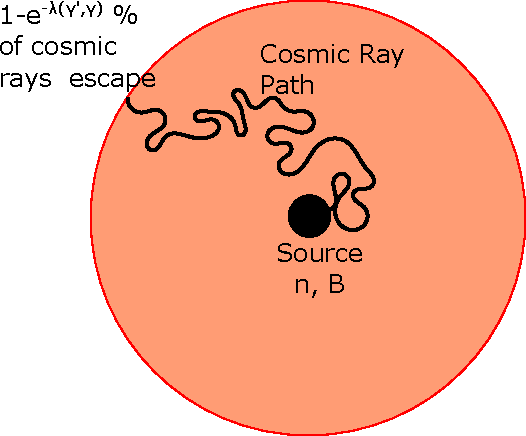
\includegraphics[width=0.6\textwidth]{07_Particle_Evolution/Images/Code/code_example.pdf}
    \caption{An accelerator inside a uniform region of ISM with number density $n$ and magnetic field $B$. After injection, cosmic rays scatter off magnetic field turbulence resulting in net diffusion from the accelerator. The probability that a cosmic ray escapes the region while cooling from Lorentz factor $\gamma'\rightarrow\gamma$ is $1-\exp(-\lambda(\gamma',\gamma))$ (see \autoref{eq:chapter_7_lambda_escape_rate})}
    \label{fig:chapter_7_code_example}
\end{SCfigure}

Cosmic rays scatter of magnetic field turbulence, randomising their direction (see \autoref{chapter_1_cr_propagation}). The net transport of cosmic rays can be described by diffusion. After time $t$, the 3D distance that approximately $68\%$ of cosmic rays have `diffused' from the accelerator is given by:

\begin{equation}
    \begin{aligned}
        R_{68\%}=6\qty(\gamma,B)Dt\text{ ,}
    \end{aligned} \label{eq:chapter_7_6Dt}
\end{equation}
\noindent where $D$ is the diffusion coefficient described in \autoref{eq:diffusion} \citep{1996A&A...309..917A}. Therefore, cosmic rays can escape the system as shown in \autoref{fig:chapter_7_code_example}. For a spherical region with radius $R$, the escape rate (particles/s) is defined to be:

\begin{equation}
    \begin{aligned}
    \nu_\text{esc}\qty(\gamma)&=\frac{6D\qty(\gamma,B)}{R^2}\text{ ,}
    \end{aligned} \label{eq:chapter_7_escape_rate}
\end{equation}
\noindent where the diffusion coefficient ($D\qty(\gamma,B)\propto \gamma^\delta $) can lie within three different regimes describing the rate of diffusion (Bohm: $\delta=1$, Kraichnan: $\delta=1/2$ and Kolmogrov $\delta =1/3$) (see \autoref{chapter_1_cr_propagation}). \noindent For Bohm diffusion ($\delta=1$), the diffusion coefficient is related to its gyro-radius ($r_g$) through:

\begin{equation}
    \begin{aligned}
    D\qty(\gamma,B)&=\frac{r_gc}{3} \\
    &=\frac{\gamma m_e c}{e B}\text{ .}
    \end{aligned}
\end{equation}
\noindent Combining \autoref{eq:diffusion} and \autoref{eq:chapter_7_escape_rate} gives:

\begin{equation}
    \begin{aligned}
    \nu_\text{esc}&=\frac{6\chi_0D_0}{R^2 (B/3)^\delta} \gamma^\delta \\
    &\equiv b_\text{esc} \gamma^\delta\text{ .}
    \end{aligned} \label{eq:chapter_7_escape_rate_2}
\end{equation}

\begin{figure}[htbt]
    \centering
    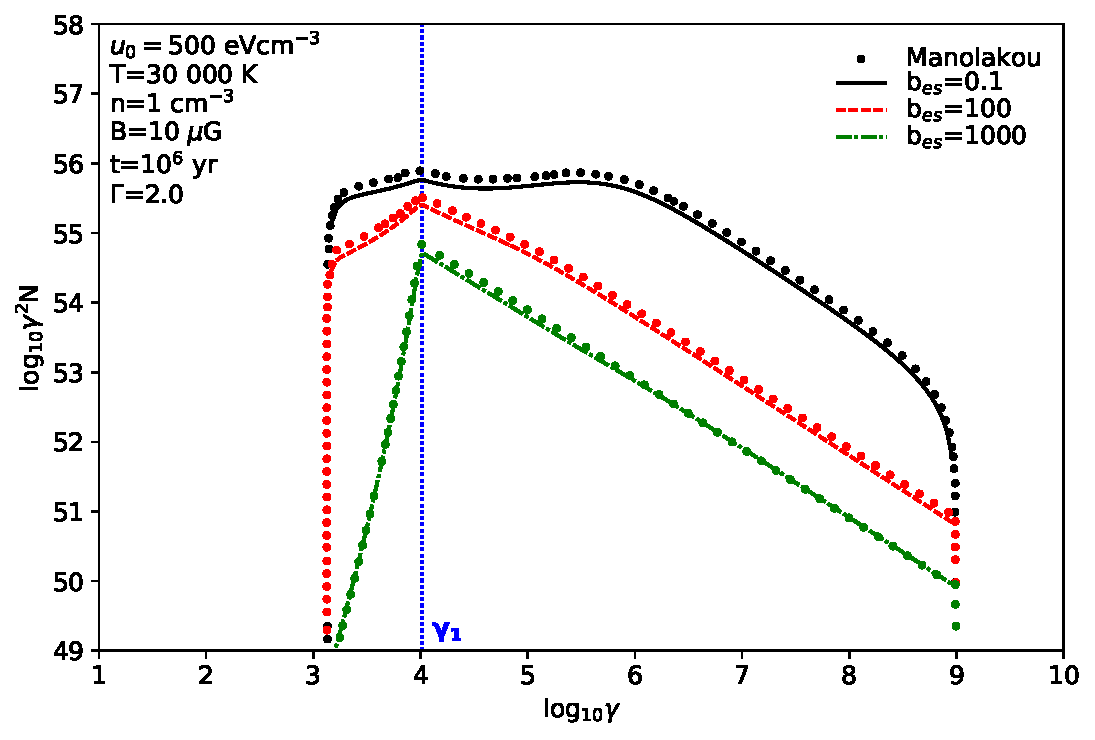
\includegraphics[width=\textwidth]{07_Particle_Evolution/Images/Code/manolakou_ecape.pdf}
    \caption{Comparison of {\tt Newsedprod} (solid lines) to results by \cite{2007A&A...474..689M} where electrons are allowed to escape the system at rate $\nu_\text{esc}= b_\text{es}\gamma$ (see \autoref{eq:chapter_7_escape_rate_2}), i.e. Bohm diffusion regime. Electrons are injected with a power-law spectrum $\Gamma=2.0$. The position of $\gamma_1$ is represented by the vertical dotted line.}
    \label{fig:chapter_7_manolakou_escape}
\end{figure}

For simplicity, synchrotron losses will be assumed to be dominant ($\dot{\gamma}=b_s\gamma^2$). Therefore, the probability that a cosmic ray escapes the region whilst cooling from $\gamma'$ to $\gamma$ is given by:

\begin{equation}
    \begin{aligned}
   	 \lambda\qty(\gamma,\gamma')&=\frac{b_\text{esc}}{b_s}\int_\gamma^{\gamma'}\dd{\gamma''}\gamma^{\delta-2} \\
  	  &=b_\text{es}
  	  \begin{cases}
  		  \ln\qty({\gamma'}/{\gamma}))\text{,}\quad &\delta =1 \\
  		  \frac{1}{\delta-1}\qty(\gamma'^{\delta-1}-\gamma^{\delta -1})\text{,}\quad&\text{otherwise}
    	\end{cases}\text{ ,}
    \end{aligned} \label{eq:chapter_7_lambda_plus_diffusion}
\end{equation}
\noindent with $b_\text{es}\equiv b_\text{esc}/b_s$. For Bohm diffusion ($\delta=1$), the probability of escape for an electron then becomes:

\begin{equation}
    \begin{aligned}
    p_\text{esc}&=1-\exp(-b_\text{es}\ln\qty(\gamma'/\gamma)) \\
    &=1-\qty(\frac{\gamma'}{\gamma})^{b_\text{es}}\text{ .}
    \end{aligned}
\end{equation}
\par~\par
\autoref{fig:chapter_7_manolakou_escape} shows the comparison of the electron energy density distribution of {\tt Newsedprod} to the results  by \cite{2007A&A...474..689M} for different values of $b_\text{es}$ assuming Bohm diffusion ($\delta=1$). There is negligible escape when $b_\text{es}=0.1$, but escape losses become significant when $b_\text{es}=100$ and $1000$. Electrons with Lorentz factor $\gamma_1$, the maximum Lorentz factor that electrons injected at $t=0$ can take, is the least affected by escape losses. Electrons with Lorentz factor $>\gamma_1$ represent the population of electrons injected after $t=0$. As the Lorentz factor increases beyond $\gamma_1$, electrons rapidly escape the region and only recently injected electrons contribute to the energy spectrum. Below $\gamma_1$, the electron cooling rate rapidly decreases and the probability that an electron escapes before cooling increases. 

\subsection{Investigation of magnetic field turbulence regimes}

\begin{figure}[hbtp]
    \centering
    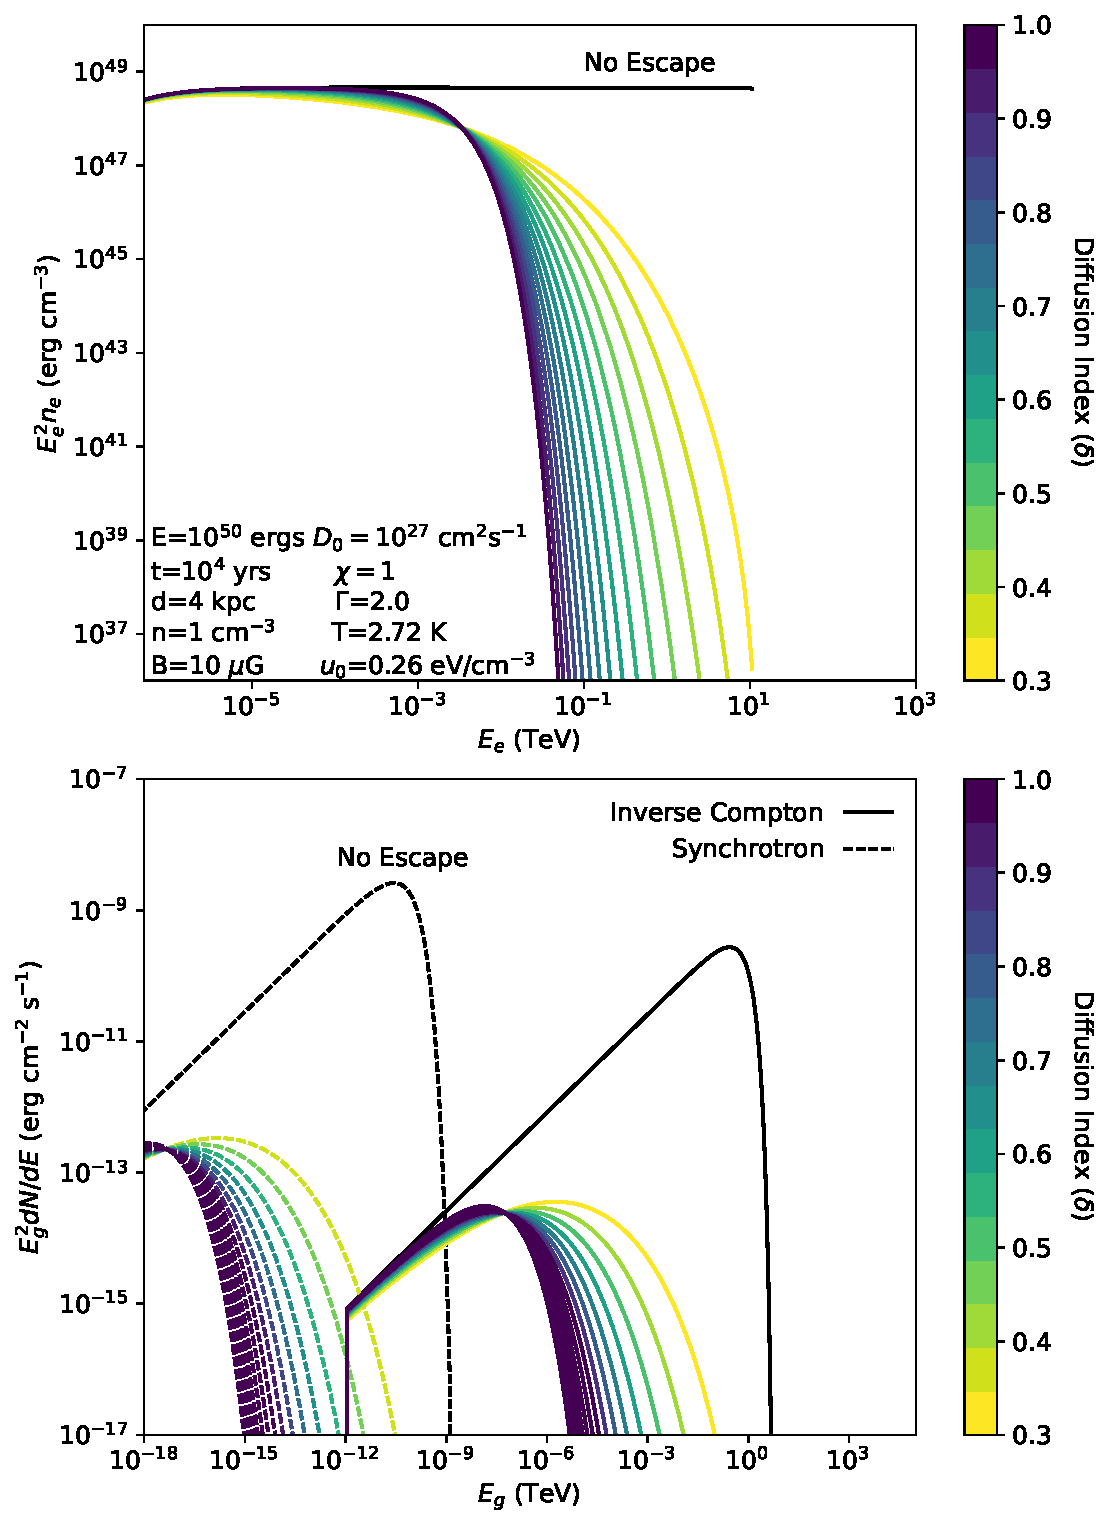
\includegraphics[width=0.9\textwidth]{07_Particle_Evolution/Images/Code/diffusion_regimes_impulsive.pdf}
    \caption{Variation of the electron energy density distribution (\textit{top}) and subsequent synchrotron and inverse Compton SED (\textit{bottom}) for an impulsive source of electrons escaping a cloud with radius $10~\pc$ in the different diffusion regimes ($\delta$). Kolmogrov regime: $\delta=\frac{1}{3}$, Kraichnan regime: $\delta=0.5$ and Bohm regime: $\delta=1$. Electrons are injected following a power law spectrum with $\Gamma=2$. The black line represents a situation where there is no escape of electrons.}
    \label{fig:chapter_7_newsedprod_diffusion_regimes_impulsive}
\end{figure}

\begin{figure}[hbtp]
    \centering
    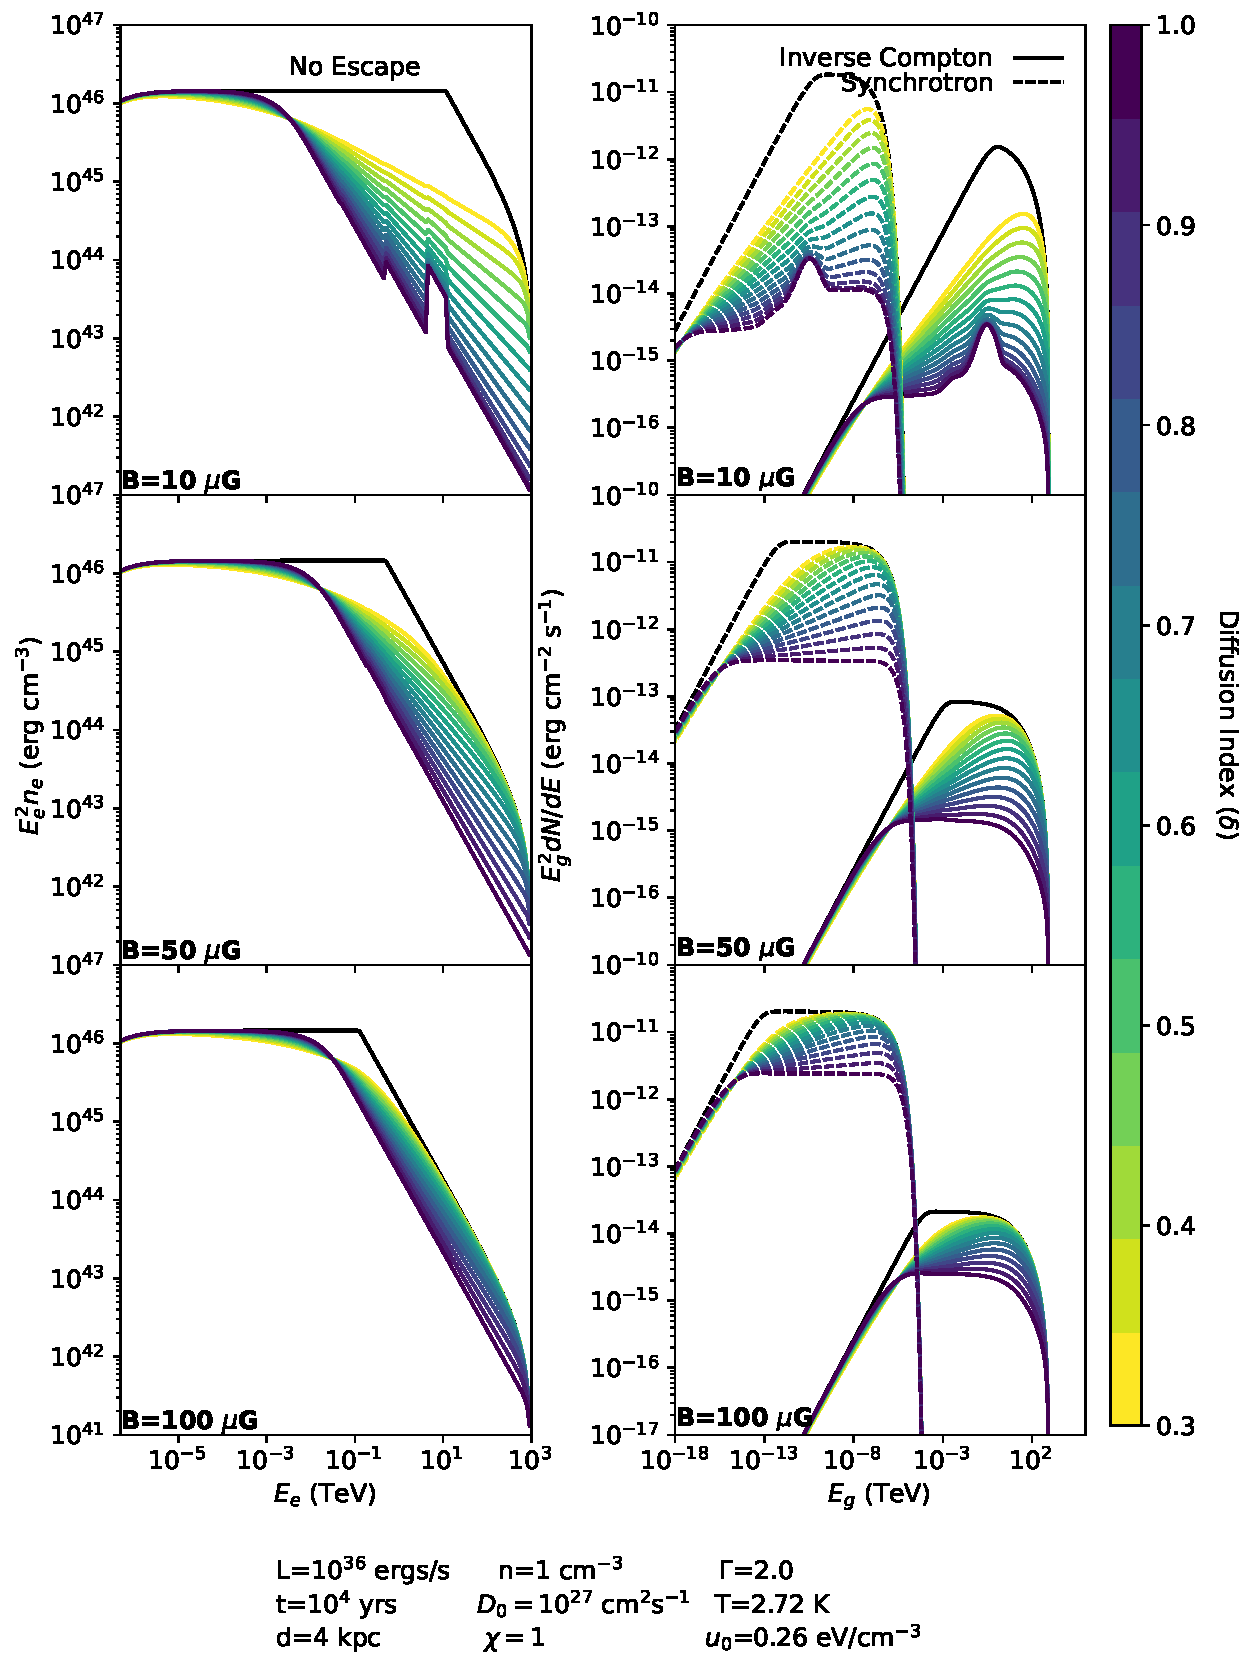
\includegraphics[width=1.0\textwidth]{07_Particle_Evolution/Images/Code/diffusion_regimes_continuous.pdf}
    \caption{Variation of the electron energy density distribution (\textit{left}) and subsequent synchrotron and inverse Compton SED (\textit{right}) for a continuous source of electrons escaping a cloud with radius $10~\pc$ in the different diffusion regimes ($\delta$). Kolmogrov regime: $\delta=\frac{1}{3}$, Kraichnan regime: $\delta=0.5$ and Bohm regime: $\delta=1$. A magnetic field of $10~\si{\micro G}$ (\textit{top}), $50~\si{\micro G}$ (\textit{middle}) and $100~\si{\micro G}$ (bottom) was utilised. The black line represents a situation where there is no escape of electrons.}
    \label{fig:chapter_7_newsedprod_diffusion_regimes_continuous}
\end{figure}

The rate at which cosmic rays escape a sphere of radius $R$ depends on the diffusion properties which, in turn, depend on the power spectrum of the magnetic field turbulence (see \autoref{eq:diffusion}). Using {\tt Newsedprod}, the effects of the different magnetic field regimes (Kolmogrov $\delta=\frac{1}{3}$, Kraichan $\delta=0.5$ and Bohm $\delta=1$) on the electron energy spectra and subsequent SED can be seen in \autoref{fig:chapter_7_newsedprod_diffusion_regimes_impulsive} and \autoref{fig:chapter_7_newsedprod_diffusion_regimes_continuous} for an impulsive and continuous electron accelerator respectively.
\par~\par 
For both accelerators types, as the power spectrum of the magnetic field turbulence ($\delta$) increases, the rate of diffusion increases for electrons $>E_\text{cr}$ and decreases for electrons $<E_\text{cr}$, where $E_\text{cr}$ is the crossover energy corresponding to $D=\chi D_0$ (see \autoref{eq:diffusion}):
\begin{equation}
    \begin{aligned}
        E_\text{cr}&=\frac{B}{3~\si{\micro G}}\quad\qty[\GeV]\text{ .}
    \end{aligned}
\end{equation}
\noindent For a magnetic field of $10~\si{\micro G}$, the cross-over energy is $0.3~\GeV$ as seen in the top panel of \autoref{fig:chapter_7_newsedprod_diffusion_regimes_impulsive}. As the magnetic field increases, the crossover energy migrates to higher energies as seen in the left hand panels of \autoref{fig:chapter_7_newsedprod_diffusion_regimes_continuous}. The subsequent IC and synchrotron SED then follows the electron energy density distribution as shown in the bottom panel of \autoref{fig:chapter_7_newsedprod_diffusion_regimes_impulsive} and right hand panels of \autoref{fig:chapter_7_newsedprod_diffusion_regimes_continuous} (see \autoref{sec:chapter_1_leptonic_gre}).
\par~\par 
Electrons will cool to a lower energy before escaping the system when their cooling time ($\tau$) is less than the time it takes for a particle to diffuse distance $R$ (see \autoref{eq:chapter_7_6Dt}). Therefore, for a continuous source, electrons with high energy reach a steady state where radiative losses and escape loses are balanced by the injected electrons (e.g. $E\gtrsim 10~\TeV$ for $B=50~\si{\micro G}$)

\subsection{Applications of {\tt Newsedprod}}

In summary, {\tt} Newsedprod numerically solves the energy density distribution of cosmic rays (protons and electrons) for an accelerator (impulsive or continuous) injecting cosmic rays into a region of constant number density, magnetic field and photon field (e.g. CMB, infra-red fields and optical photons). {\tt Newsedprod} can then be tuned (e.g. changing the injected spectra or age of the system) to sources such as PWNe and SNRs to compare the predicted SED to observations from instruments such as HE.S.S. and \textit{Fermi}-LAT (see \autoref{sec:02_TeV_observatories}). Observatories such as Nanten (see \autoref{sec:NANTEN}) can be used to obtain information about the number density of hydrogen towards the object of interest and estimate the magnetic field strength through Crutcher's relation (see \autoref{eq:ISM_crutchers} and \cite{2010ApJ...725..466C}). Once the model `matches' the observed emission from the source, the input parameter space can be examined to see if the model is reasonable or not.
\par~\par
\autoref{sec:08} applies {\tt Newsedprod} to a region south of the PWNe \mbox{HESS\,J1825-137} in order to determine the origin of cosmic rays resulting in the $\GeV$ emission seen towards this region. It was postulated that either an accelerator associated with \mbox{HESS\,J1825-137} (PWN or the progenitor SNR) or with nearby binary system \mbox{LS\,5039} (accretion onto associated compact object or progenitor SNR) powered the $\GeV$ emission. Using {\tt Newsedprod}, it was found that neither source provided sufficient energetics to account for this emission, but did not rule out a combination of both sources.